%%%%&latex
\documentclass[11pt]{article}
\usepackage{amsmath, bm, amssymb, amsthm, mathrsfs}
\usepackage[bb=boondox]{mathalfa}
\usepackage{paralist}
\usepackage{natbib}
\usepackage{url}
\usepackage{multirow, booktabs, float, textcmds, siunitx}
\usepackage{todonotes}
\usepackage{qtree, tikz}
\usetikzlibrary{arrows,positioning,shapes,fit,calc}
\usepackage{graphicx}
\usepackage[section]{placeins}
\usepackage{algorithm, algorithmicx, algpseudocode}
%\pdfminorversion=4
% NOTE: To produce blinded version, replace "0" with "1" below.
\newcommand{\blind}{1}

% DON'T change margins - should be 1 inch all around.
\addtolength{\oddsidemargin}{-.5in}%
\addtolength{\evensidemargin}{-.5in}%
\addtolength{\textwidth}{1in}%
\addtolength{\textheight}{1in}%
\addtolength{\topmargin}{-.8in}%

\usepackage{caption}
\DeclareCaptionStyle{italic}[justification=centering]
 {labelfont={bf},textfont={it},labelsep=colon}
\captionsetup[figure]{style=italic,format=hang,singlelinecheck=true}
\captionsetup[table]{style=italic,format=hang,singlelinecheck=true}

\DeclareMathOperator*{\argmin}{arg\,min}
\newcolumntype{L}{>{$}l<{$}} % math-mode version of "l" column type

\def\E{\text{E}}
\def\var{\text{Var}}
\def\PQ{\bigg(\begin{matrix}\bm{G}\\[-0.2cm]\bm{G}_{\perp}^-\end{matrix}\bigg)}
\def\bt{\bigg(\begin{matrix}\bm{b}\\[-0.2cm]\bm{a}\end{matrix}\bigg)}

%\theoremstyle{theo}
\newtheorem{theo}{Theorem}[section]

\theoremstyle{definition}
\newtheorem{definition}{Definition}[section]

\begin{document}

	\def\spacingset#1{\renewcommand{\baselinestretch}%
		{#1}\small\normalsize} \spacingset{1}

	%%%%%%%%%%%%%%%%%%%%%%%%%%%%%%%%%%%%%%%%%%%%%%%%%%%%%%%%%%%%%%%%%%%%%%%%%%%%%%

	\if1\blind
	{
		\title{\textbf{Probabilistic Forecast Reconciliation: Properties, Evaluation and Score Optimisation }}
		        \author{
			    Anastasios Panagiotelis\thanks{
			    	The authors gratefully acknowledge the support of Australian Research Council Grant DP140103220. We also thank Professor Mervyn Silvapulle for valuable comments.}\hspace{.2cm}\\
			    Department of Econometrics and Business Statistics,\\
		    	Monash University,\\ VIC 3800, Australia.\\
			    Email: anastasios.panagiotelis@monash.edu \\
			    and \\
			    Puwasala Gamakumara\\
			    Department of Econometrics and Business Statistics,\\
			    Monash University,\\ VIC 3800, Australia.\\
			    Email: puwasala.gamakumara@monash.edu \\
			    and \\
		        George Athanasopoulos\\
		        Department of Econometrics and Business Statistics,\\
		        Monash University,\\ VIC 3800, Australia.\\
		        Email: george.athanasopoulos@monash.edu \\
		        and \\
	            Rob J Hyndman\\
	            Department of Econometrics and Business Statistics,\\
	            Monash University,\\ VIC 3800, Australia.\\
	            Email: rob.hyndman@monash.edu \\}
		\maketitle
	} \fi

	\if0\blind
	{
		\bigskip
		\bigskip
		\bigskip
		\begin{center}
			{\LARGE\textbf{Probabilistic Forecasts for Hierarchical~Time~Series}}
		\end{center}
		\medskip
	} \fi

	\bigskip

\newpage

\begin{abstract}
We develop a framework for prediction of multivariate data that follow some known linear constraints, such as the example where some variables are aggregates of others. This is particularly common when forecasting time series (predicting the future), but also arises in other types of prediction. For point prediction, an increasingly popular technique is reconciliation, whereby predictions are made for all series (so-called `base' predictions) and subsequently adjusted to ensure coherence with the constraints. This paper extends reconciliation from the setting of point prediction to probabilistic prediction. A novel definition of reconciliation is developed and used to construct densities and draw samples from a reconciled probabilistic prediction. In the elliptical case, it is proven that the true predictive distribution can be recovered from reconciliation even when the location and scale matrix of the base prediction are chosen arbitrarily. To find reconciliation weights, an objective function based on scoring rules is optimised. The energy and variogram scores are considered since the log score is improper in the context of comparing unreconciled to reconciled predictions, a result also proved in this paper. To account for the stochastic nature of the energy and variogram scores, optimisation is achieved using stochastic gradient descent. This method is shown to improve base predictions in simulation studies and in an empirical application, particularly when the base prediction models are severely misspecified. When misspecification is not too severe, extending popular reconciliation methods for point prediction can result in a similar performance to score optimisation via stochastic gradient descent. The methods described here are implemented in the \emph{ProbReco} package for R.
\end{abstract}

\noindent%
\emph{Keywords:} Scoring Rules, Probabilistic Forecasting, Hierarchical Time Series, Stochastic Gradient Descent.
%\vfill

\newpage
\spacingset{1.45} % DON'T change the spacing!

\section{Introduction}\label{sec:intro}

Many multivariate prediction problems involve data that follow some linear constraints. For instance, in retail or tourism it is important to forecast demand in individual regions as well as aggregate demand of a whole country. In recent years reconciliation has become an increasingly popular method for handling such problems \citep[see][for an overview]{FPP2018}. Reconciliation involves producing predictions for all variables and making a subsequent adjustment to ensure these adhere to known linear constraints. While this methodology has been extensively developed for point prediction, there is a paucity of literature dealing with probabilistic predictions. This paper develops a formal framework for probabilistic reconciliation, derives theoretical results that allow reconciled probabilistic forecasts to be constructed and evaluated, and proposes an algorithm for optimally reconciling probabilistic forecasts with respect to a proper scoring rule.

Before describing the need for probabilistic reconciliation we briefly review the literature on point forecast\footnote{Such has been the dominance of forecasting in the literature on reconciliation, that we will refer to forecasting throughout the remainder of the paper. However, we note that the techniques discussed throughout the paper generalise to prediction problems in general and are not limited to time series.} reconciliation. Prior to the development of forecast reconciliation, the focus was on finding a subset of variables that could be subsequently aggregated or disaggregated to find forecasts for all series \citep[see][and references therein]{Dunn1976,Gross1990}. An alternative approach emerged with \cite{AthEtAl2009} and \cite{HynEtAl2011} who recommended producing forecasts of all series and then adjusting, or `reconciling', these forecasts to be `coherent', i.e. adhere to the aggregation constraints. These papers formulated reconciliation as a regression model, however subsequent work has formulated reconciliation as an optimisation problem where weights are chosen to minimise a loss, such as a weighted squared error \citep{VanErven2015a,nystrup2020}, a penalised version thereof \citep{bentaiebkoo}, or the trace of the forecast error covariance \citep{WicEtAl2019}.

In contrast to the point forecasts, the entire probability distribution of future values provides a full description of the uncertainty associated with the predictions \citep{Abramson1995, Gneiting2014}. Therefore probabilistic forecasting has become of great interest in many disciplines such as, economics \citep{zarnowitz1987, rossi2014}, meteorological studies \citep{pinson2009, mclean2013}, energy forecasting \citep{wytock2013, BenTaieb2017} and retail forecasting \citep{bose2017}. An early attempt towards probabilistic forecast reconciliation came from \cite{ShaHyn2017} who applied reconciliation to forecast quantiles, rather than to the point forecasts, in order to construct prediction intervals. This idea was extended to constructing a full probabilistic forecast by \citet{JeoEtAl2019} who propose a number of algorithms, one of which is equivalent to reconciling a large number of forecast quantiles. \citet{Taieb2017} also propose an algorithm to obtain probabilistic forecasts that cohere to linear constraints. In particular, \citet{Taieb2017} draw a sample from the probabilistic forecasts of univariate models for the bottom level data, reorder these to match the empirical copula of residuals, and aggregate these in a bottom-up fashion. The only sense in which top level forecasts are used is in the mean, which is adjusted to match that obtained using the MinT reconciliation method \citep{WicEtAl2019}.

There are a number of shortcomings to \citet{JeoEtAl2019} and \citet{Taieb2017} which to the best of our knowledge represent the only attempts to develop algorithms for probabilistic forecast reconciliation. First, little formal justification is provided for the algorithms, or for the sense in which they generalise forecast reconciliation to the probabilistic domain. As such, both algorithms are based on sampling and neither can be used to obtain a reconciled density analytically. Both algorithms are tailored towards specific applications and conflate reconciliation with steps that involve reordering the base forecasts. For example, while \citet{JeoEtAl2019} show that ranking draws from independent base probabilistic forecasts before reconciliation is effective, this may only be true due to the highly dependent time series considered in their application. A limitation of \citet{Taieb2017} is that to ensure their sample from the base probabilistic forecast has the same empirical copula as the data, it must be of the same size as the training data. This will be problematic in applications with fewer observations than the smart meter data they consider. Further, \citet{Taieb2017} only incorporate information from the forecast mean of aggregate variables, missing out on potentially valuable information in the probabilistic forecasts of aggregate data.

In this paper we seek to address a number of open issues in probabilistic forecast reconciliation. First, we develop in a formal way, definitions and a framework that generalise reconciliation from the point setting to the probabilistic setting. This is achieved by extending the geometric framework proposed by \cite{PanEtAl2020_Geometry} for point forecast reconciliation. Second, we utilise these definitions to show how a reconciled forecast can be constructed from an arbitrary base forecast. Solutions are provided in the case where a density of the base probabilistic forecast is available and in the case where it is only possible to draw a sample from the base forecasting distribution. Third, we show that in the elliptical case, the correct predictive distribution can be recovered via linear reconciliation irrespective of the location and scale parameters of the base forecasts. We also derive conditions for when this also holds for the special case of reconciliation via projection. Fourth, we derive theoretical results on the evaluation of reconciled probabilistic forecasts using multivariate scoring rules, including showing that the log score is improper when used to compare reconciled to unreconciled forecasts. Fifth, we propose an algorithm for choosing reconciliation weights by optimising a scoring rule. This algorithm takes advantage of advances in stochastic gradient descent and is thus suited to scoring rules that are themselves often only known up to an approximation. The algorithm and other methodological contributions described in this paper are implemented in the \emph{ProbReco} package \citep{RProbReco}.

The remainder of the paper is structured as follows. In Section~\ref{sec:ProbForecasts}, after a brief review of point forecast reconciliation, novel definitions are provided for coherent forecasts and reconciliation in the probabilistic setting. In Section~\ref{sec:AnalyticalSolution}, we outline how reconciliation can be achieved in both the case where the density of the base probabilistic forecast is available, and in the case where a sample has been generated from the base probabilistic forecast. In Section~\ref{sec:evaluation}, we consider the evaluation of probabilistic hierarchical forecasts via scoring rules, including theoretical results on the impropriety of the log score in the context of forecast reconciliation. The use of scoring rules motivates our algorithm for finding optimal reconciliation weights using stochastic gradient descent, which is described in Section~\ref{sec:scoreoptSGD} and evaluated in an extensive simulation study in Section~\ref{sec:simulations}. An empirical application on forecasting electricity generation from different sources is contained in Section~\ref{sec:Application}. Finally Section~\ref{sec:conclusion} concludes with some discussion and thoughts on future research.

\section{Hierarchical probabilistic forecasts}\label{sec:ProbForecasts}

Before introducing coherence and reconciliation to the probabilistic setting, we first briefly refresh these concepts in the case of point forecasts. In doing so, we follow the geometric interpretation introduced by \cite{PanEtAl2020_Geometry}, since this formulation naturally generalises to probabilistic forecasting.

\subsection{Point Forecasting}\label{sec:PointForecasts}

A \emph{hierarchical time series} is a collection of time series adhering to some known linear constraints. Stacking the value of each series at time $t$ into an $n$-vector $\bm{y}_t$, the constraints imply that $\bm{y}_t$ lies in an $m$-dimensional linear subspace of $\mathbb{R}^n$ for all $t$. This subspace is referred to as the \emph{coherent subspace} and is denoted as $\mathfrak{s}$. A typical (and the original) motivating example is a collection of time series some of which are aggregates of other series. In this case $\bm{b}_t \in \mathbb{R}^m$ can be defined as the values of the most disaggregated or \emph{bottom-level series} at time $t$ and the aggregation constraints can be formulated as,
\begin{equation*}
	\bm{y}_t = \bm{S}\bm{b}_t,
\end{equation*}
where $\bm{S}$ is an $n \times m$ constant matrix for a given hierarchical structure.

\begin{figure}[!htb]
	\begin{center}
		\leaf{AA} \leaf{AB}
		\branch{2}{A}
		\leaf{BA} \leaf{BB}
		\branch{2}{B}
		\branch{2}{Tot}
		\qobitree
	\end{center}
	\caption{An example of a two-level hierarchical structure.}\label{fig:twoL-hier}
\end{figure}
An example of a hierarchy is shown in Figure~\ref{fig:twoL-hier}. There are $n=7$ series of which $m=4$ are bottom-level series. Also, $\bm{b}_t = [y_{AA,t}, y_{AB,t}, y_{BA,t}, y_{BB,t}]'$, $\bm{y}_t = [y_{Tot,t},y_{A,t}, y_{B,t},\bm{b}'_t]'$, and
\[
\bm{S} = \begin{pmatrix}
1 & 1 & 1 & 1 \\
1 & 1 & 0 & 0 \\
0 & 0 & 1 & 1 \\
& \multicolumn{2}{c}{\bm{I}_4} &
\end{pmatrix},
\]
where $\bm{I}_4$ is the $4\times 4$ identity matrix.

The connection between this characterisation and the coherent subspace is that the columns of $\bm{S}$ span $\mathfrak{s}$. Below, the notation $s:\mathbb{R}^m\rightarrow\mathbb{R}^n$ is used when premultiplication by $\bm{S}$ is thought of as a mapping. Finally, while $\bm{S}$ is defined in terms of $m$ bottom-level series here, in general any $m$ series can be chosen with the $\bm{S}$ matrix redefined accordingly. The columns of all appropriately defined $\bm{S}$ matrices span the same coherent subspace $\mathfrak{s}$.

When forecasts of all $n$ series are produced, they may not adhere to constraints. In this case forecasts are called \emph{incoherent base} forecasts and are denoted $\hat{\bm{y}}_{t+h}$, with the subscript $t+h$ implying a $h$-step-ahead forecast at time $t$. To exploit the fact that the target of the forecast adheres to known linear constraints, these forecasts can be adjusted in a process known as \emph{forecast reconciliation}. At its most general, this involves selecting a mapping $\psi:\mathbb{R}^n\rightarrow\mathfrak{s}$ and then setting $\tilde{\bm{y}}_{t+h}=\psi(\hat{\bm{y}}_{t+h})$, where $\tilde{\bm{y}}_{t+h}\in\mathfrak{s}$ is called the \emph{reconciled} forecast. The mapping $\psi$ may be considered as the composition of two mappings $\psi=s\circ g$. Here, $g:\mathbb{R}^{n}\rightarrow\mathbb{R}^{m}$ combines incoherent base forecasts of all series to produce new bottom-level forecasts, which are then aggregated via $s$. Many existing point forecasting approaches including the bottom-up \citep{Dunn1976}, OLS \citep{HynEtAl2011}, WLS \citep[][]{Hyndman2016,AthEtAl2017} and MinT \citep{WicEtAl2019} methods, are special cases where $g$ involves premultiplication by a matrix $\bm{G}$ and where $\bm{S}\bm{G}$ is a projection matrix. These are summarised in Table~\ref{tab:ReconMethods}.

\begin{table}[!t]
	\caption{Summary of reconciliation methods for which $\bm{S}\bm{G}$ is a projection matrix. Here $\bm{W}$ is some diagonal matrix, $\hat{\bm{\Sigma}}_{\text{sam}}$ is a sample estimate of the residual covariance matrix and $\hat{\bm{\Sigma}}_{\text{shr}}$ is a shrinkage estimator proposed by \citet{Schafer2005}, given by $\tau \textrm{diag}(\hat{\bm{\Sigma}}_{\text{sam}})+(1-\tau)\hat{\bm{\Sigma}}_{\text{sam}}$ where $\tau = \displaystyle\frac{\sum_{i \neq j}\hat{\var}(\hat{\sigma}_{ij})}{\sum_{i \neq j}{\hat{\sigma}}^2_{ij}}$ and $\sigma_{ij}$ denotes the $(i,j)$th element of $\hat{\bm{\Sigma}}_{\text{sam}}$.} \label{tab:ReconMethods}
	\centering
	\begin{tabular}{l@{\hskip 0.4in}l}
		\toprule
		\textbf{Reconciliation method} & $\bm{G}$ \\
		\midrule
		OLS             & $(\bm{S}'\bm{S})^{-1}\bm{S}'$ \\
		WLS             & $(\bm{S}'\bm{W}\bm{S})^{-1}\bm{S}'\bm{W}$ \\
		MinT(Sample)    & $(\bm{S}'\hat{\bm{\Sigma}}_{\text{sam}}^{-1}\bm{S})^{-1}\bm{S}' \hat{\bm{\Sigma}}_{\text{sam}}^{-1}$  \\
		MinT(Shrink)    & $(\bm{S}'\hat{\bm{\Sigma}}_{\text{shr}}^{-1}\bm{S})^{-1}\bm{S}' \hat{\bm{\Sigma}}_{\text{shr}}^{-1}$  \\
		\bottomrule
	\end{tabular}
	\label{tab:recomethods}
\end{table}

\subsection{Coherent probabilistic forecasts}

We now turn our attention towards a novel definition of coherence in a probabilistic setting. First let $(\mathbb{R}^m, \mathscr{F}_{\mathbb{R}^m}, \nu)$ be a probability triple, where $\mathscr{F}_{\mathbb{R}^m}$ is the usual Borel $\sigma$-algebra on $\mathbb{R}^m$. This triple can be thought of as a probabilistic forecast for the bottom-level series. A $\sigma$-algebra $\mathscr{F}_{\mathfrak{s}}$ can then be constructed as the collection of sets $s(\mathcal{B})$ for all $\mathcal{B}\in \mathscr{F}_{\mathbb{R}^m}$, where $s(\mathcal{B})$ denotes the image of $\mathcal{B}$ under the mapping $s$.

\begin{definition}[Coherent Probabilistic Forecasts]\label{def:cohprob}
	Given the triple, $(\mathbb{R}^m, \mathscr{F}_{\mathbb{R}^m}, \nu)$, a coherent probability triple $(\mathfrak{s}, \mathscr{F}_{\mathfrak{s}}, \breve{\nu})$, is given by $\mathfrak{s}$, the $\sigma$-algebra $\mathscr{F}_{\mathfrak{s}}$ and a measure $\breve{\nu}$, such that
	\[
	\breve{\nu}(s(\mathcal{B})) = \nu(\mathcal{B}) \quad \forall \mathcal{B} \in \mathscr{F}_{\mathbb{R}^m}.
	\]
\end{definition}

To the best of our knowledge, the only other definition of coherent probabilistic forecasts is given by \cite{Taieb2017} who define them in terms of convolutions. While these definitions do not contradict one another, our definition has two advantages. First it can more naturally be extended to problems with non-linear constraints with the coherent subspace $\mathfrak{s}$ replaced with a manifold. Second, it facilitates a definition of probabilistic forecast reconciliation to which we now turn our attention.

\subsection{Probabilistic forecast reconciliation}

Let $(\mathbb{R}^n, \mathscr{F}_{\mathbb{R}^n}, \hat{\nu})$ be a probability triple characterising a probabilistic forecast for all $n$ series. The hat is used for $\hat{\nu}$ analogously with $\hat{\bm{y}}$ in the point forecasting case. The objective is to derive a reconciled measure $\tilde{\nu}$, assigning probability to each element of the $\sigma$-algebra $\mathscr{F}_\mathfrak{s}$.

\begin{definition} \label{def:reconprob}
	The reconciled probability measure of $\hat{\nu}$ with respect to the mapping $\psi(.)$ is a probability measure $\tilde{\nu}$ on $\mathfrak{s}$ with $\sigma$-algebra $\mathscr{F}_\mathfrak{s}$ such that
	\[
	\tilde{\nu}(\mathcal{A}) = \hat{\nu}(\psi^{-1}(\mathcal{A})) \qquad \forall \mathcal{A} \in \mathscr{F}_{\mathfrak{s}}\,,
	\]
	where $\psi^{-1}(\mathcal{A}):=\{{\bm{y}}\in \mathbb{R}^n:\psi({\bm{y}})\in \mathcal{A}\}$ is the pre-image of $\mathcal{A}$, that is the set of all points in $\mathbb{R}^n$ that $\psi(.)$ maps to a point in $\mathcal{A}$.
\end{definition}

This definition naturally extends forecast reconciliation to the probabilistic setting. In the point forecasting case, the reconciled forecast is obtained by passing an incoherent forecast through a transformation. Similarly, for probabilistic forecasts, sets of points is mapped to sets of points by a transformation. The same probabilities are assigned to these sets under the base and reconciled measures respectively. Recall that the mapping $\psi$ can also be expressed as a composition of two transformations $s\circ g$. In this case, an $m$-dimensional reconciled probabilistic distribution $\nu$ can be obtained such that $\nu(\mathcal{B})= \hat{\nu}(g^{-1}(\mathcal{B}))$ for all $\mathcal{B} \in \mathscr{F}_{\mathbb{R}^m}$ and a probabilistic forecast for the full hierarchy can then be obtained via Definition~\ref{def:cohprob}. This construction will be used in Section~\ref{sec:AnalyticalSolution}.

Definition~\ref{def:reconprob} can use any continuous mapping $\psi$, where continuity is required to ensure that open sets in $\mathbb{R}^n$ used to construct $\mathscr{F}_{\mathbb{R}^n}$ are mapped to open sets in $\mathfrak{s}$. However, hereafter, we restrict our attention to $\psi$ as a linear mapping. This is depicted in Figure~\ref{fig:probfr_sch} when $\psi$ is a projection. This figure is only a schematic, since even the most trivial hierarchy is $3$-dimensional. The arrow labelled $\bm{S}$ spans an $m$-dimensional coherent subspace $\mathfrak{s}$, while the arrow labelled $\bm{R}$ spans an $(n-m)$-dimensional direction of projection. The mapping $g$ collapses all points in the blue shaded region $g^{-1}(\mathcal{B})$, to the black interval $\mathcal{B}$. Under $s$, $\mathcal{B}$ is mapped to $s(\mathcal{B})$ shown in red. Under our definition of reconciliation, the same probability is assigned to the red region under the reconciled measure as is assigned to the blue region under the incoherent measure.

\begin{figure}[!htb]
	\centering 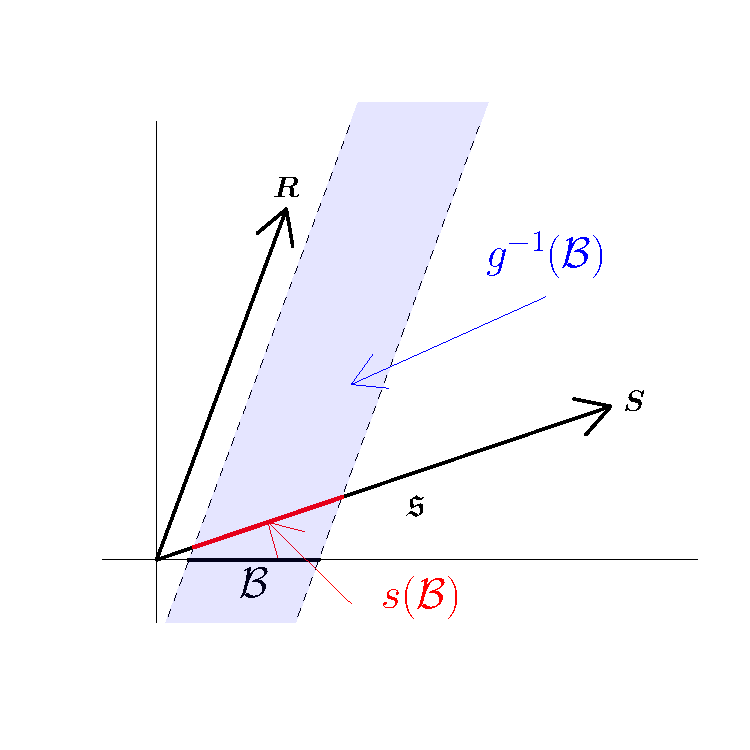
\includegraphics[width=0.5\textwidth]{Figs/probforerec_schematic.pdf}
	\caption{Summary of probabilistic forecast reconciliation. The probability that $\bm{y}_{t+h}$ lies in the red line segment under the reconciled probabilistic forecast is defined to be equal to the probability that $\bm{y}_{t+h}$ lies in the shaded blue area under the unreconciled probabilistic forecast. Note that since the smallest possible hierarchy involves three dimensions, this figure is only a schematic.}\label{fig:probfr_sch}
\end{figure}

\section{Construction of Reconciled Distribution} \label{sec:AnalyticalSolution}

In this section we derive theoretical results on how distributions on $\mathbb{R}^n$ can be reconciled to a distribution on $\mathfrak{s}$. In Section~\ref{sec:andens} we show how this can be achieved analytically by a change of coordinates and marginalisation when the density is available. In Section~\ref{sec:elliptical} we explore this result further in the specific case of elliptical distributions. In Section~\ref{sec:SampleSolution} we consider reconciliation in the case where the density may be unavailable but it is possible to draw a sample from the base probabilistic forecast distribution. Throughout we restrict our attention to linear reconciliation.

\subsection{Analytical derivation of reconciled densities}\label{sec:andens}

The following theorem shows how a reconciled density can be derived from any base probabilistic forecast on $\mathbb{R}^n$.

\begin{theo}[Reconciled density of bottom-level]\label{theo:bottomdens}
	Consider the case where reconciliation is carried out using a composition of linear mappings $s\circ g$ where $g$ combines information from all levels of the base forecast into a new density for the bottom-level. The density of the bottom-level series under the reconciled distribution is
	\[
	\tilde{f}_{\bm{b}}(\bm{b})=|\bm{G}^*|\int \hat{f}(\bm{G}^{-}\bm{b}+\bm{G}_\perp \bm{a})d\bm{a}\,,
	\]
	where $\hat{f}$ is the density of the incoherent base probabilistic forecast, $\bm{G^-}$ is an $n\times m$ generalised inverse of $\bm{G}$ such that $\bm{G}\bm{G}^-=\bm{I}$, $\bm{G_\perp}$ is an $n\times (n-m)$ orthogonal complement to $\bm{G}$ such that $\bm{G}\bm{G}_\perp=\bm{0}$, $\bm{G}^*=\left(\bm{G}^-\,\vdots\,\bm{G}_\perp\right)$, and $\bm{b}$ and $\bm{a}$ are obtained via the change of variables
	\[
	\bm{y}=\bm{G}^*\begin{pmatrix}\bm{b}\\\bm{a}\end{pmatrix}\,.
	\]
\end{theo}

\begin{proof}
	See Appendix~\ref{app:Bottom&FullDens}.
\end{proof}

\begin{theo}[Reconciled density of full hierarchy]\label{theo:fulldens}
	Consider the case where a reconciled density for the bottom-level series has been obtained using Theorem~\ref{theo:bottomdens}. The density of the full hierarchy under the reconciled distribution is
	\[
	\tilde{f}_{\bm{y}}(\bm{y}) =
	|\bm{S}^*| \tilde{f}_{\bm{b}}({\bm{S}^-\bm{y}})
	\mathbb{1}\{\bm{y}\in\mathfrak{s}\}\,,
	\]
	where $\mathbb{1}\{\cdot\}$ equals $1$ when the statement in braces is true and 0 otherwise,
	\[
	\bm{S}^*=\begin{pmatrix}
	\bm{S}^-\\
	\bm{S}'_\perp
	\end{pmatrix}\,,
	\]
	$\bm{S^-}$ is an $m\times n$ generalised inverse of $\bm{S}$ such that $\bm{S}^-\bm{S}=\bm{I}$,
	and $\bm{S_\perp}$ is an $n\times (n-m)$ orthogonal complement to $\bm{S}$ such that $\bm{S}'_\perp\bm{S}=\bm{0}$.
\end{theo}

\begin{proof}
	See Appendix~\ref{app:Bottom&FullDens}.
\end{proof}

\subsubsection*{Example: Gaussian Distribution}

Suppose the incoherent base forecasts are Gaussian with mean $\hat{\bm{\mu}}$, covariance matrix $\hat{\bm{\Sigma}}$ and density,
\begin{equation}
\hat{f}(\hat{y})=(2\pi)^{-n/2}|\hat{\bm{\Sigma}}|^{-1/2}\exp\left\{-\frac{1}{2}\left[({\bm{y}}-\hat{\bm{\mu}})'\hat{\bm{\Sigma}}^{-1}({\bm{y}}-\hat{\bm{\mu}})\right]\right\}\nonumber.
\end{equation}
Then, using Theorem~\ref{theo:bottomdens}, the reconciled density for the bottom-level series is given by
\begin{equation}
\tilde{f}_{\bm{b}}(\bm{b})=\int(2\pi)^{-\frac{n}{2}}|\hat{\bm{\Sigma}}|^{-\frac{1}{2}}|\bm{G}^*|e^{-q/2} d\bm{a}\nonumber\,,
\end{equation}
where
\begin{align*}
	q& =
	\bigg[\bm{G}^*\bt-\hat{\bm{\mu}}\bigg]' \hat{\bm{\Sigma}}^{-1}\bigg[\bm{G}^*\bt-\hat{\bm{\mu}}\bigg]\\
	& =
	\bigg[\bt-\bm{G}^{*-1}\hat{\bm{\mu}}\bigg]'
	\bigg[\bm{G}^{*-1}\hat{\bm{\Sigma}}(\bm{G}^{*-1})'\bigg]^{-1}
	\bigg[\bt-\bm{G}^{*-1}\hat{\bm{\mu}}\bigg]\,.
\end{align*}
Noting that
\[
\bm{G}^{*-1}=\Bigg(\begin{matrix}
\bm{G} \\\bm{G}_{\perp}^-
\end{matrix}\Bigg)\,,
\]
where $\bm{G}_{\perp}^-$ is an $(n-m)\times n$ matrix such that $\bm{G}_{\perp}^-\bm{G}_{\perp}=\bm{I}$, $q$ can be rearranged as
\[
\bigg[\bt-\PQ\hat{\bm{\mu}}\bigg]'
\bigg[\PQ\hat{\bm{\Sigma}}\PQ'\bigg]^{-1}
\bigg[\bt-\PQ\hat{\bm{\mu}}\bigg]\,.
\]
After the change of variables, the density can be recognised as a multivariate Gaussian in $\bm{b}$ and $\bm{a}$. The mean and covariance matrix for the margins of the first $m$ elements are $\bm{G}\hat{\bm{\mu}}$ and $\bm{G}\hat{\bm{\Sigma}}\bm{G}'$ respectively. Marginalising out $\bm{a}$, the reconciled forecast for the bottom-level is $\tilde{\bm{b}} \sim \mathcal{N}(\bm{G}\hat{\bm{\mu}}, \bm{G}\hat{\bm{\Sigma}}\bm{G}')$. Using standard results from matrix algebra of normals, $\tilde{\bm{y}} \sim \mathcal{N}(\bm{S}\bm{G}\hat{\bm{\mu}}, \bm{S}\bm{G}\hat{\bm{\Sigma}}\bm{G}'\bm{S}')$.

\subsection{Elliptical distributions}\label{sec:elliptical}

More generally, consider linear reconciliation of the form $\psi(\hat{\bm{y}})=\bm{S}(\bm{d}+\bm{G}\hat{\bm{y}})$. For an elliptical base probabilistic forecast, with location $\hat{\bm\mu}$ and scale $\hat{\bm\Sigma}$, the reconciled probabilistic forecast will also be elliptical with location $\tilde{\bm{\mu}}=\bm{S}(\bm{d}+\bm{G}\hat{\bm{\mu}})$ and scale $\tilde{\bm{\Sigma}}=\bm{S}\bm{G}\hat{\bm{\Sigma}}\bm{G}'\bm{S}'$. This is a consequence of the fact that elliptical distributions are closed under linear transformations and marginalisation. While the base and reconciled distribution may be of a different form, they will both belong to the elliptical family. This leads to the following result.

\begin{theo}[Recovering the true density through reconciliation]\label{theo:OptRec}
	Assume the true predictive distribution is elliptical with location ${\bm\mu}$ and scale ${\bm\Sigma}$. Then for an elliptical base probabilistic forecast with arbitrary location $\hat{\bm\mu}$ and scale $\hat{\bm\Sigma}$, there exists $\bm{d}_{\text{opt}}$ and $\bm{G}_{\text{opt}}$ such that the true predictive distribution is recovered by reconciliation.
\end{theo}
\begin{proof}
	First consider finding a $\bm{G}_{\text{opt}}$ for which the following holds,
	\begin{equation*}
		\bm{\Sigma}=\bm{S}\bm{G}_{\text{opt}}\hat{\bm{\Sigma}}\bm{G}'_{\text{opt}}\bm{S}'\,.
	\end{equation*}
	This can be solved as $\bm{G}_{\text{opt}}=\bm{\Omega}_0^{1/2}\hat{\bm{\Sigma}}^{-1/2}$, where $\hat{\bm{\Sigma}}^{1/2}$ is any matrix such that $\hat{\bm{\Sigma}}=\hat{\bm{\Sigma}}^{1/2}(\hat{\bm{\Sigma}}^{1/2})'$ (for example a Cholesky factor), ${\bm{\Omega}}_0^{1/2}({\bm{\Omega}}_0^{1/2})'={\bm\Omega}$ and ${\bm\Omega}$ is the true scale matrix for the bottom-level series. To ensure conformability of matrix multiplication, ${\bm{\Omega}}^{1/2}$ must be an $m\times n$ matrix; so it can be set to the Cholesky factor of ${\bm{\Omega}}$ augmented with an additional $n-m$ columns of zeros. To reconcile the location, solve the following for $\bm{d}_{\text{opt}}$
	\begin{equation*}
		\bm{\mu}=\bm{S}(\bm{d}_{\text{opt}}+\bm{G}_{\text{opt}}\hat{\bm{\mu}})\,
	\end{equation*}
	which is given by $\bm{d}_{\text{opt}}=\bm{\beta}-\bm{G}_{\text{opt}}\hat{\bm\mu}$, where $\bm{\beta}$ is defined so that $\bm{\mu}=\bm{S}\bm{\beta}$.
\end{proof}

While the above theorem is not feasible in practice (exploiting the result requires knowledge of $\bm{\mu}$ and $\bm{\Sigma}$), it does nonetheless have important consequences for the algorithm that we introduce in Section~\ref{sec:scoreoptSGD}. In particular, note that $\bm{S}\bm{G}_{\text{opt}}$ is not a projection matrix in general. This implies that in the probabilistic forecasting setting, it is advised to include a translation $\bm{d}$ in the reconciliation procedure. This holds even if the base forecasts are unbiased (i.e. $\hat{\bm{\mu}}=\bm{\mu}$) since in general $\bm{S}\bm{G}_{\text{opt}}\hat{\bm{\mu}}\neq\bm{\mu}$.

Although $\bm{S}\bm{G}_{\text{opt}}$ is not a projection matrix in general, there are some conditions under which it will be. These are described by the following theorem.
\begin{theo}[Optimal Projection for Reconciliation]\label{theo:OptRecProj}
	Let $\hat{\bm{\Sigma}}$ be the scale matrix from an elliptical but incoherent base forecast and assume base forecasts are also unbiased. When the true predictive distribution is also elliptical, then this can be recovered via reconciliation using a projection if $\textrm{rank}(\hat{\bm{\Sigma}}-\bm{\Sigma})\leq n-m$.
\end{theo}
\begin{proof}
	See Appendix~\ref{app:OptRecProj}.
\end{proof}

\subsection{Simulation from a Reconciled Distribution}\label{sec:SampleSolution}

In practice it is often the case that samples are drawn from a probabilistic forecast since an analytical expression is either unavailable, or relies on unrealistic parametric assumptions. A useful result is the following.
\begin{theo}[Reconciled samples]
	Suppose that $\left(\hat{\bm{y}}^{[1]},\ldots,\hat{\bm{y}}^{[L]}\right)$ is a sample drawn from an incoherent probability measure $\hat{\nu}$. Then $\left(\tilde{\bm{y}}^{[1]},\ldots,\tilde{\bm{y}}^{[L]}\right)$ where $\tilde{\bm{y}}^{[\ell]}:=\psi(\hat{\bm{y}}^{[\ell]})$ for $\ell=1,\ldots,L$, is a sample drawn from the reconciled probability measure $\tilde{\nu}$ as defined in Definition~\ref{def:reconprob}.
\end{theo}
\begin{proof}
	For any $\mathcal{A}\in\mathscr{F}_{\mathfrak{s}}$
	\begin{align}
		\mbox{Pr}(\hat{\bm{y}}\in\psi^{-1}(\mathcal{A}))&=\underset{L\rightarrow\infty}{\lim}\sum\limits_{\ell=1}^L\mathbb{1}\big\{\hat{\bm{y}}^{[\ell]}\in\psi^{-1}(\mathcal{A})\big\}\nonumber\\
		&=\underset{L\rightarrow\infty}{\lim}\sum\limits_{\ell=1}^L\mathbb{1}\big\{\psi(\hat{\bm{y}}^{[\ell]})\in(\mathcal{A})\big\}\nonumber\\
		&=\mbox{Pr}(\tilde{\bm{y}}\in(\mathcal{A}))\nonumber
	\end{align}
\end{proof}

This result implies that reconciling each member of a sample drawn from an incoherent distribution provides a sample from the reconciled distribution. Such a strategy has already been used by \cite{JeoEtAl2019}, without formal justification. This result allows coherent forecasts to be built in a general and modular fashion, the mechanism for simulating base forecasts is separated from the question of reconciliation. This will become clear in the simulation study covered in Section~\ref{sec:simulations}.


\section{Evaluation of Hierarchical Probabilistic Forecasts} \label{sec:evaluation}

An important issue in all forecasting problems is evaluating forecast accuracy. In the probabilistic setting, it is common to evaluate forecasts using proper scoring rules \citep[see][and references therein]{Gneiting2007,Gneiting2014}. Throughout, we follow the convention of negatively oriented scoring rules such that smaller values of the score indicate more accurate forecasts. In general, a scoring rule $K(.,.)$, is a function taking a probability measure as the first argument and a realisation as the second argument (although for ease of notation we will at times replace the probability measure with its associated density in the first argument). A scoring rule is \emph{proper} if $\E_{Q}[K(Q,\bm{\omega})] \le \E_{Q}[K(P,{\bm\omega})]$ for all $P$, where $P$ is any member of some class of probability measures (densities), $Q$ is the true predictive and $\bm{\omega}$ is a realisation. When this inequality is strict for all $P\neq Q$, the scoring rule is said to be \emph{strictly proper}.

Since hierarchical forecasting is inherently a multivariate problem (the linear constraints affect all variables), our focus is on multivariate scoring rules. Arguably the simplest and most common multivariate scoring rule is the log score. The log score simply involves evaluating the negative log density at the value of the realisation, $\text{LS}(P,\bm\omega)=-\log f(\bm\omega)$, where $f$ is the density associated with a distribution $P$. The log score is more commonly used when a parametric form for the density is available, however this density can also be approximated from a sample of values drawn from the probabilistic forecast \citep[see][]{Jordan2017}.

Alternatively there are a number of other multivariate scoring rules that are difficult to compute using the probabilistic forecast density alone, but can be approximated using a sample drawn from that density. An example is the energy score (ES) \citep[see][for details]{szekely2003,Gneiting2007} which is a multivariate generalisation of the popular Cumulative Rank Probability Score (CRPS). The energy score is given by
\begin{equation}\label{eq:Energy_score}
\text{ES}(P,\bm{\omega}) =
\E_{P}
||{\bm{y}}-\bm{\omega}||^\alpha -\frac{1}{2}\E_{P}||\bm{y}-\bm{y}^*||^\alpha, \,\, \alpha \in (0,2]\,,
\end{equation}
where $\bm{y}$ and $\bm{y}^*$ are independent copies drawn from the distribution $P$. In the empirical results described later, we follow common convention by setting $\alpha=1$. While the expectations in Equation~\eqref{eq:Energy_score} may have no closed form, they can be easily approximated via simulations using a sample drawn from the probabilistic forecast. Other scores with similar behaviour are kernel-based scores \citep{dawid2007,Gneiting2007} and the variogram score \citep{SCHEUERER2015}.

\subsection{The Log Score for Hierarchical Time Series}

When an expression for the density of an incoherent base forecast is available, Section~\ref{sec:AnalyticalSolution} describes how the density of a reconciled forecast can be recovered. With both densities available, the log score is a natural and straightforward scoring rule to use. However, the following theorem shows that the log score is improper in the setting of comparing incoherent to coherent forecasts.

\begin{theo}[Impropriety of log score]\label{theo:logS_improp}
	When the true data generating process is coherent, then the log score is improper with respect to the class of incoherent measures.
\end{theo}

\begin{proof}
	See Appendix~\ref{app:logS_improp}.
\end{proof}

As a result of Theorem~\ref{theo:logS_improp} we recommend avoiding the log score when comparing reconciled and unreconciled probabilistic forecasts.

If a probabilistic forecast is available for any $m$ series, then a probabilistic forecast for the full hierarchy can be derived. Definition~\ref{def:cohprob} provides an example using the bottom-level series. This suggests that it may be adequate to merely compare two coherent forecasts to one another using the bottom-level series only. This is true for the log score.

Consider a coherent probabilistic forecast with density $\tilde{f}_{\bm{y}}$ for the full hierarchy and $\tilde{f}_{\bm{b}}$ for the bottom-level series. By Theorem~\ref{theo:fulldens}, $\tilde{f}_{\bm{y}}(\bm{y})=|\bm{S}^*|\tilde{f}_{\bm{b}}(\bm{S}^-\bm{y})\mathbb{1}\{\bm{y}\in\mathfrak{s}\}$. Any realisation $\bm{y}^*$ will lie on the coherent subspace and can be written as $\bm{S}\bm{b}^*$. The expression for the log score is therefore
\begin{align}
	\text{LS}(\tilde{f}_{\bm{y}},\bm{y}^*)&=-\log\left(|\bm{S}^*|\tilde{f}_{\bm{b}}(\bm{S}^-\bm{S}\bm{b}^*)\right)\nonumber\\
	&=-\log|\bm{S}^*|-\log \tilde{f}_{\bm{b}}(\bm{b}^*).\nonumber
\end{align}
For coherent densities, the log score for the full hierarchy differs from the log score for the bottom-level series only by $-\log|\bm{S}^*|$. This term is independent of the choice of $\bm{G}$. Consequently, rankings of different reconciliation methods using the log score for the full hierarchy will not change if only the bottom-level series is used.

The same property does not hold for all scores. For example, the energy score is invariant under orthogonal transformations \citep{Szekely2013} but not under linear transformations in general. Therefore it is possible for one method to outperform another when energy score is calculated using the full hierarchy, but for these rankings to change if only bottom-level series are considered. We therefore recommend computing the energy score using the full hierarchy. The properties of multivariate scoring rules in the context of evaluating reconciled probabilistic forecasts are summarised in Table~\ref{tab:prop}.

\begin{table}
	\caption{Properties of scoring rules for reconciled probabilistic forecasts.}\label{tab:ScoringRulesProperties}
	\centering
	\begin{tabular}{lll}\hline
		Scoring Rule& Coherent v Incoherent &Coherent v Coherent\\
		\hline
		Log Score & Not proper & Ordering preserved if compared \\ && using bottom-level only\\
		Energy Score & Proper & Full hierarchy should be used\\
		\hline
	\end{tabular}
	
	\label{tab:prop}
\end{table}

\section{Score Optimal Reconciliation}\label{sec:scoreoptSGD}

We now propose an algorithm for finding reconciliation weights by optimising an objective function based on scores. For clarity of exposition, we consider the special case of the energy score. However, the algorithm can be generalised to any score that is computed by sampling from the probabilistic forecast. For example, in the simulations and the empirical application of Sections~\ref{sec:simulations} and~\ref{sec:Application} we consider optimising with respect to both the energy and variogram scores. We consider linear reconciliation of the form $\tilde{\bm{y}}=\psi_{\bm{\gamma}}({\bm{\hat{y}}})={\bm{S}}\left(\bm{d}+\bm{G}{\bm{\hat{y}}}\right)$, where ${\bm\gamma}:=\left(\bm{d},vec(\bm{G})\right)$. This allows for more flexibility than a projection, which would imply the constraints $\bm{d}=\bm{0}$ and $\bm{G}\bm{S}=\bm{I}$. This added flexibility is motivated by Theorem~\ref{theo:OptRec} which shows that projections in general are not guaranteed to recover the true predictive distribution even in the elliptical case. When making an $h$-step-ahead forecast at time $T$, the objective used to determine an optimal value of $\bm{\gamma}$ is the total energy score based on in-sample information, given by
\begin{equation}
\mathcal{E}\left(\bm{\gamma}\right)=\sum\limits_{t=T}^{T+R-1} \textit{ES}(\tilde{f}^{\bm{\gamma}}_{t+h|t},\bm{y}_{t+h})\,,
\label{eq:tes}
\end{equation}
where $\tilde{f}^{\bm{\bm{\gamma}}}_{t+h|t}$ a is probabilistic forecast for $\bm{y}_{t+h}$ made at time $t$ and reconciled with respect to $\psi_{\bm{\gamma}}(.)$, and $R$ is the number of score evaluations used in forming the objective function.

One of the challenges in optimising this objective function is that there is, in general, no closed form expression for the energy score. However, it can be easily approximated by simulation as
\begin{equation}
\hat{\mathcal{E}}\left(\bm{\gamma}\right)=\sum\limits_{t=T}^{T+R-1}\left[\frac{1}{Q}\bigg(\sum\limits_{q=1}^{Q}||\tilde{\bm{y}}^{[q]}_{t+h|t}-\bm{y}_{t+h}||-\frac{1}{2}||\tilde{\bm{y}}_{t+h|t}^{[q]}-\tilde{\bm{y}}^{*[q]}_{t+h|t}||\bigg)\right]\,,
\label{eq:obj_mc}
\end{equation}
where $\tilde{\bm{y}}^{[q]}_{t+h|t}=\bm{S}\big(\bm{d}+\bm{G}{\hat{\bm{y}}}^{[q]}_{t+h|t}\big)$, $\tilde{\bm{y}}^{*[q]}_{t+h|t}=\bm{S}\big(\bm{d}+\bm{G}{\hat{\bm{y}}}^{*[q]}_{t+h|t}\big)$ and ${\hat{\bm{y}}}^{[q]}_{t+h|t},{\hat{\bm{y}}}^{*[q]}_{t+h|t}\overset{iid}{\sim} \hat{f}_{t+h|t}$ for $q=1,\ldots,Q$.

The objective function is optimised by Stochastic Gradient Descent (SGD). The SGD technique has become increasingly popular in machine learning and statistics over the past decade having been applied to training neural networks \citep{bottou2010} and Variational Bayes \citep{kingma2013}. The method requires an estimate of the gradient $\partial\hat{\mathcal{E}}/\partial{\gamma}$ which is computed by automatically differentiating Equation~\eqref{eq:obj_mc} using the header only C++ library of the Stan project~\citep{carpenter2015}. The learning rates used for SGD are those of the Adam method \citep[see][for details]{kingma2014}. Pseudo-code for the full procedure in the case where $h=1$ is provided in Algorithm~\ref{alg:scoreopt} and is implemented in the R package \textit{ProbReco} \citep{RProbReco}.

\begin{algorithm}[!thb]
	\caption{SGD with Adam for score optimal reconciliation (one-step-ahead forecasts). The initial value of $\bm{\gamma}$ is given by OLS reconciliation. Steps 9--14 are the standard steps for SGD with Adam. Squaring $\bm{g}_j$ in Step 11 and division and addition in Step 14 are element-wise operations.}\label{alg:scoreopt}.
	\begin{algorithmic}[1]
		\Procedure{ScoreOpt}{$\bm{y}_1,\ldots,\bm{y}_{T+R}$, $\beta_1$,$\beta_2$,$\epsilon$,$\eta$}.
		\For{$t=T:T+R-1$}
		\State Find base forecasts $\hat{f}_{t+1|t}$ using $t-T+1,t-T+2,\ldots,t$ as training data.
		\EndFor
		\State Initialise $\bm{m}_0=\bm{0}, \bm{v}_0=\bm{0}$ and $\bm{\gamma}_0=\left(\bm{0},\text{vec}\left((\bm{S}'\bm{S})^{-1}\bm{S}'\right)\right)$
		\For{$j = 1,2,3,\ldots$ up to convergence}
		\State Draw ${\hat{\bm{y}}}^{[q]}_{t+1|t},{\hat{\bm{y}}}^{*[q]}_{t+1|t}\sim \hat{f}_{t+1|t}$ for $q=1,\ldots,Q$, $t=T,\ldots T+R-1$.
		\State Compute $\tilde{\bm{y}}^{[q]}_{t+1|t}$ and $\tilde{\bm{y}}^{*[q]}_{t+1|t}$ for $q=1,\ldots,Q$, $t=T,\ldots T+R-1$ using $\bm{\gamma}_{j-1}$.
		\State $\bm{g}_j \gets \left.\partial\hat{\mathcal{E}}/\partial{\bm{\gamma}}\right|_{\bm{\gamma}=\bm{\gamma}_{j-1}}$ \Comment{Compute gradient}
		\State $\bm{m}_j\gets\beta_1\bm{m}_{j-1}+(1-\beta_1)\bm{g}_j$ \Comment{Moving average of gradient}
		\State $\bm{v}_j\gets\beta_2\bm{v}_{j-1}+(1-\beta_2)\bm{g}^2_j$ \Comment{Moving average of squared gradient}
		\State $\hat{\bm{m}}_j\gets \bm{m}_j/(1-\beta_1^j)$ \Comment{Bias correct}
		\State $\hat{\bm{v}}_j\gets \bm{v}_j/(1-\beta_2^j)$ \Comment{Bias correct}
		\State $\bm{\gamma}_j\gets\bm{\gamma}_{j-1}+\eta\frac{\hat{\bm{m}}_j}{(\hat{\bm{v}}_j+\epsilon)}$ \Comment{Update weights}
		\EndFor
		\State Set the reconciled forecast as $\tilde{f}^{\bm{\gamma}_{\text{opt}}}_{T+R+1|T+R}$ where $\bm{\gamma}_{\text{opt}}$ is the converged value of $\bm{\gamma}$.
		\EndProcedure
	\end{algorithmic}
\end{algorithm}

While Algorithm~\ref{alg:scoreopt} is not the first instance of calibrating parameters by optimising scoring rules \citep[see][for an earlier example]{gneiting2005}, to the best of our knowledge it is the first instance of doing so using SGD and the first application to forecast reconciliation. It is amenable to parallel computing architectures: the loop beginning at line 2 of the pseudo-code of Algorithm~\ref{alg:scoreopt} can be done in parallel as can the computation of the gradient. Finally, the total score in Equation~\eqref{eq:tes} can be replaced with a weighted sum where appropriate; for instance weights that decay for scores computed further in the past will favour choices of $\bm{\gamma}$ that produced better forecasting performance for more recent forecast windows.

\section{Simulations}\label{sec:simulations}

The aim of the simulations that follow is to demonstrate probabilistic forecast reconciliation including the algorithm discussed in Section~\ref{sec:scoreoptSGD}. For all simulations, the tuning parameters for the SGD are set as $\eta=0.001$, $\beta_1=0.9$, $\beta_2=0.999$ and $\epsilon=1\times 10^{-8}$, which are the values recommended by \cite{kingma2014} and used in popular software packages such as TensorFlow, Keras and Torch amongst others. Convergence is achieved when the change in all gradients is less than 10\% of the step size $\eta$. The number of sample periods used to construct the objective function is $R=250$, while the number of draws used to estimate each score is $Q=250$. All estimation of base models uses a sample size of $T=500$. All forecast evaluations are carried out using a rolling window, also of size $W=500$.

\subsection{Data Generating Processes}\label{sec:dgp}

The data generating process we consider corresponds to the 3-level hierarchical structure presented in Figure~\ref{fig:twoL-hier}. Bottom-level series are first generated from ARIMA$(p,d,q)$ processes, which are in turn aggregated to form the middle and top-level series. The orders $p$ and $q$ are randomly selected from $\{1,2\}$ for each bottom-level series. The AR and MA parameters are randomly and uniformly generated from $[0.3,0.5]$ and $[0.3,0.7]$ respectively, and only accepted if they belong to the stationary and invertible region. In addition a non-stationary case where $d$ is randomly chosen for each bottom-level from $\{0,1\}$ was considered, these results are omitted for brevity. A complete set of results are available at the github repository \url{https://git.io/JJwQB}.

We consider a multivariate Gaussian and a non-Gaussian setting for the errors driving the ARIMA processes. Specifically, the non-Gaussian errors are drawn from a meta-distribution of a Gumbel copula with $\text{Beta}(1,3)$ margins. After simulating from the ARIMA models, additional noise is added to ensure bottom-level series have a lower signal-to-noise ratio than top level series with details provided in Appendix~\ref{app:DGP}. For each series the first 500 observations are ignored to avoid the impact of initial values.


\subsection{Modelling and Base Forecasts}

We fit univariate ARIMA models to each series using the \verb|ARIMA()| function in the \verb|fable| package \citep{Rfable} in R \citep{Rcore}. Note that the order of the ARIMA models is not set to the true order but is chosen using the algorithm of \cite{HynKha2008}, allowing for the possibility of misspecification. Indeed, an advantage of forecast reconciliation is the ability to down-weight the forecasts of series within the hierarchy that come from misspecified models. We also considered exponential smoothing (ETS) models using the \verb|ETS()| function in the \verb|fable| package. These are omitted for brevity; please refer to \url{https://git.io/JJwQB} for a full set of results.

Let $\hat{\bm{y}}_{t+h|t}=\left(\hat{y}_{1,t+h|t},\ldots,\hat{y}_{n,t+h|t}\right)'$, where $\hat{y}_{i,t+h|t}$ is the $h$-step-ahead point forecast for series $i$, and $\bm{E}:=\left\{e_{i,t}\right\}_{i=1,\dots,n;t=1,\dots,T}$ is an $(n \times T)$ matrix of stacked residuals $e_{i,t}$. For each series and model, base probabilistic forecasts for $h=1$ are constructed in the following four ways:
\begin{compactitem}
	\item \textbf{Independent Gaussian:} The base probabilistic forecast is made up of independent Gaussian distributions with the forecast mean and variance of variable $i$ given by $\hat{y}_{i,t+h|t}$ and $\hat{\sigma}^2_{i,t+h|t}$, where $\hat{\sigma}^2_{i,t+h|t}$ is the sample variance of the residuals in the $i$th row of $\bm{E}$.
	\item \textbf{Joint Gaussian:} The base probabilistic forecast is a multivariate Gaussian distribution with the forecast mean $\hat{\bm{y}}_{t+h|t}$ and variance covariance matrix $\hat{\bm\Sigma}$, where $\hat{\bm\Sigma}$ is the variance covariance matrix of the residuals.
	\item \textbf{Independent Bootstrap:} A draw from the base probabilistic forecast is made independently for each variable as $\hat{y}_{i,t+h|t}+e_{i,\tau}$ where $\tau$ is drawn randomly (with replacement) from $1,2,\ldots, T$.
	\item \textbf{Joint Bootstrap:} A draw from the joint probabilistic forecast is made as $\hat{\bm{y}}_{t+h|t}+\bm{e}_{\tau}$ where $\bm{e}_{\tau}$ is the $\tau$th column of $\bm{E}$, where $\tau$ is drawn randomly (with replacement) from $1,2,\ldots, T$.
\end{compactitem}

We restrict our attention to the case of $h=1$ although these methods can be generalised to larger $h$ using the recursive method \citep{FPP2018}. For multi-step-ahead forecasts, methods (c) and (d) should be sampled in blocks to preserve serial dependence in the residuals.

\subsection{Reconciliation}

For each DGP, model and method for obtaining base forecasts, reconciled probabilistic forecasts are obtained using each of the following techniques.
\begin{compactitem}
	\item \textbf{Base:} The base forecasts with no reconciliation.
	\item \textbf{JPP:} The best method of \cite{JeoEtAl2019}. This is equivalent to reconciling quantiles. A sample is drawn from the base forecast, these are ranked, one variable at a time (so that the smallest value drawn from each variable are put together, etc.). These are then pre-multiplied by $\bm{S}\left(\bm{S}'\bm{W}\bm{S}\right)^{-1}\bm{S}'\bm{W}$ where $\bm{W}$ is a diagonal matrix with elements ($1/4^2$,$1/2^2$,$1/2^2$,$1$,$1$,$1$,$1$). These are the squared reciprocals of the number of bottom-level series used to form an aggregate.
	\item \textbf{BTTH:} The method of \cite{Taieb2017}. This is a method whereby draws from the probabilistic forecasts of the bottom-level series are permuted so that they have the same empirical copula as the residuals. These are then aggregated to form a sample from the distribution of all series. The mean is adjusted to be equivalent to the mean that would be obtained using the MinT method of \cite{WicEtAl2019} described in Table~\ref{tab:recomethods}.
	\item \textbf{BottomUp:} Reconciliation via premultiplication by $\bm{S}\bm{G}$ where $\bm{G}=\left(\bm{0}_{m\times(n-m)},\bm{I}_{m\times m}\right)$.
	\item \textbf{OLS:} Reconciliation via pre-multiplication by $\bm{S}\left(\bm{S}'\bm{S}\right)^{-1}\bm{S}'$.
	\item \textbf{MinTShr:} Reconciliation via pre-multiplication using the shrinkage estimator of the covariance matrix used by \cite{WicEtAl2019} but applied to probabilistic rather than point forecasting.
	\item \textbf{ScoreOptE:} The algorithm described in Section~\ref{sec:scoreoptSGD} used to optimise energy score.
	\item \textbf{ScoreOptV:} The algorithm described in Section~\ref{sec:scoreoptSGD} used to optimise variogram score.
\end{compactitem}

Note that JPP and BTTH are two methods previously existing in the literature. The methods BottomUp, OLS, and MinTShr have been used extensively in the point forecasting literature but their application to probabilistic forecasting for general base forecasts is, to the best of our knowledge, novel in this paper.

In addition to these methods, two further reconciliation methods were considered; WLS, which reconciles via pre-multiplication by the same matrix used in \cite{JeoEtAl2019} but without any reordering of the draws, and MinTSam which uses a sample estimate of the covariance matrix rather than a shrinkage estimator. These methods were mostly dominated by OLS and MinTShr respectively and are therefore omitted for brevity; please refer to \url{https://git.io/JJwQB} for a full set of results.

\subsection{Results for Gaussian probabilistic forecasts}\label{sec:SimAnalysticalResults}

The left panel of Figure~\ref{fig:meanscore_g} shows the mean energy score for different reconciliation methods and different methods of generating base forecasts. When base probabilistic forecasts are generated independently, score optimisation with the energy score (ScoreOptE) performs best, while when base forecasts are generated jointly, the MinT method for reconciliation using the shrinkage estimator (MinTShr) yields the most accurate forecasts. The bottom-up method as well as BTTH and JPP fail to even improve upon base forecasts in all cases. As expected score optimisation using the variogram score does not perform as well as score optimisation using energy score, when evaluation is carried out with respect to the latter. However, the results are quite close suggesting that score optimisation is fairly robust to using an alternative proper score.

\begin{figure}[!htb]
	\centering
	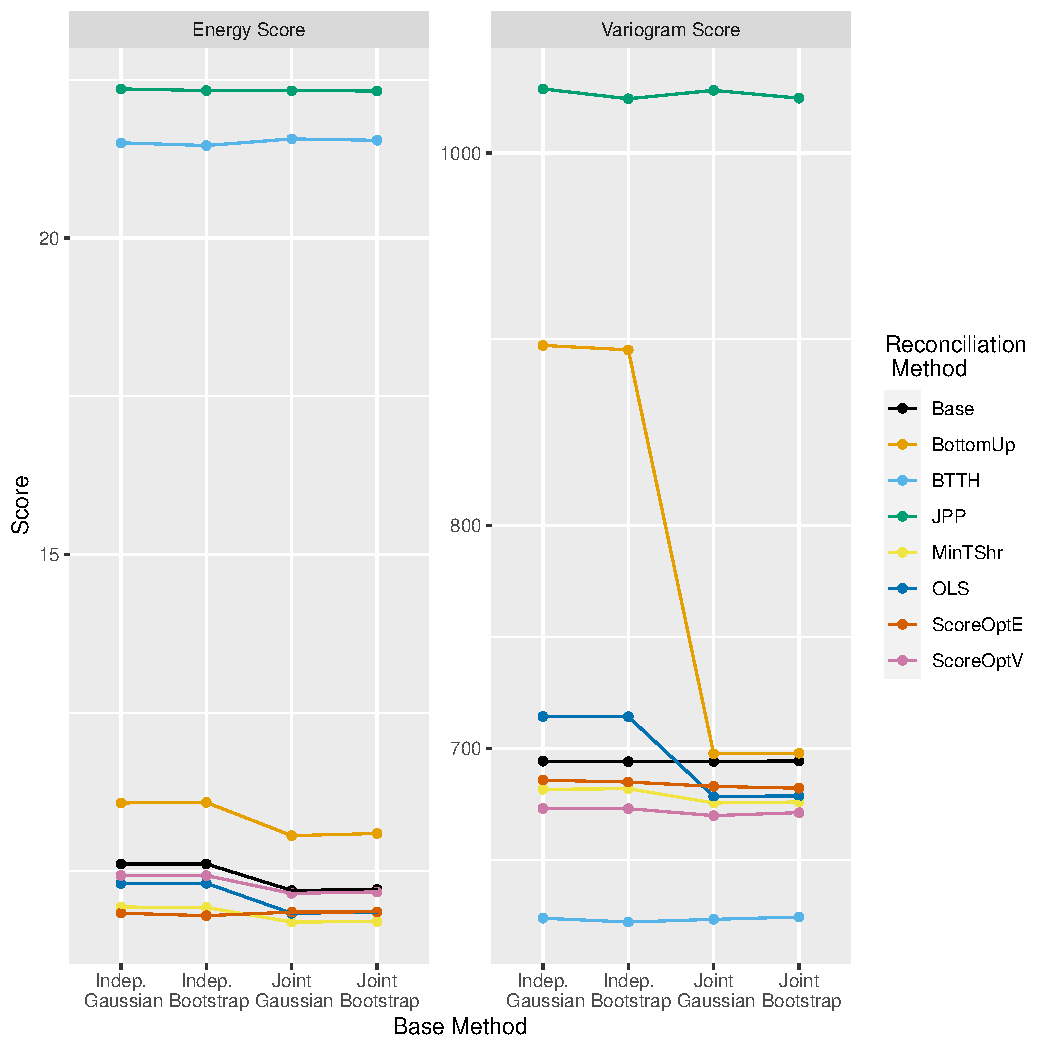
\includegraphics[width=0.85\textwidth]{Figs/gaussian_meanscore}
	\caption{Mean scores for Gaussian DGP\@ using different base forecast and reconciliation methods. The left panel is the energy score, the right panel is the variogram score.}
	\label{fig:meanscore_g}
\end{figure}

\begin{figure}[!htb]
	\centering
	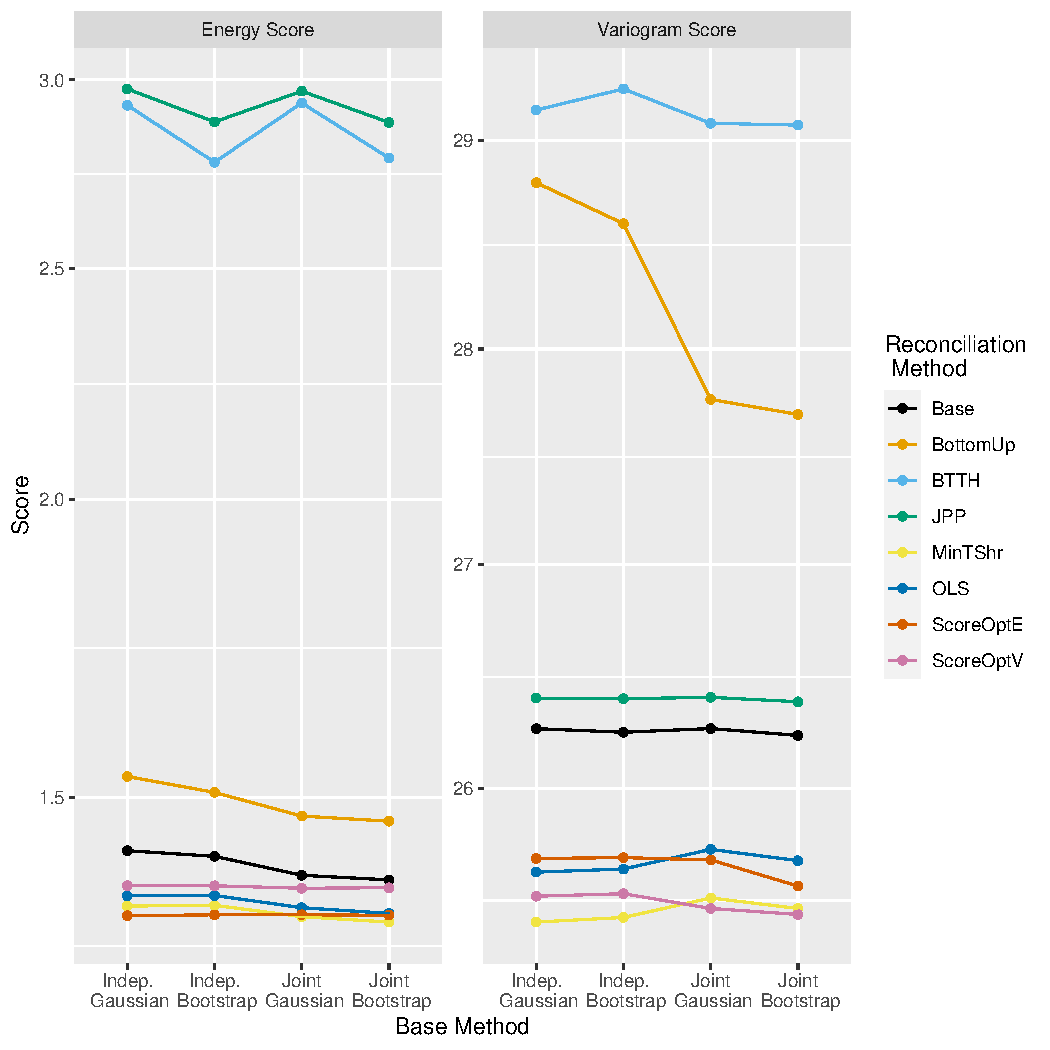
\includegraphics[width=0.85\textwidth]{Figs/nongaussian_meanscore}
	\caption{Mean scores for non-Gaussian DGP\@ using different base forecast and reconciliation methods.  The left panel is the energy score, the right panel is the variogram score.}
	\label{fig:meanscore_n}
\end{figure}

To assess significant differences between the reported results, we use post-hoc Nemenyi tests \citep{HolEtAl2013}. The Nemenyi test is a non-parametric test that identifies groups of forecasts which cannot be significantly distinguished from one another. We use the implementation of the tests available in the \verb|tsutils| R package \citep{tsutilspackage}. Figure~\ref{fig:gse} reports the results which should be looked at column-wise. A blue square indicates that the method in the corresponding row, is statistically indistinguishable from the method in that column. For all four methods of generating base forecasts, MinTShr, ScoreOptE and OLS significantly outperform base forecasts, bottom-up forecasts, BTTH and JPP.


\begin{figure}[!htb]
	\centering
	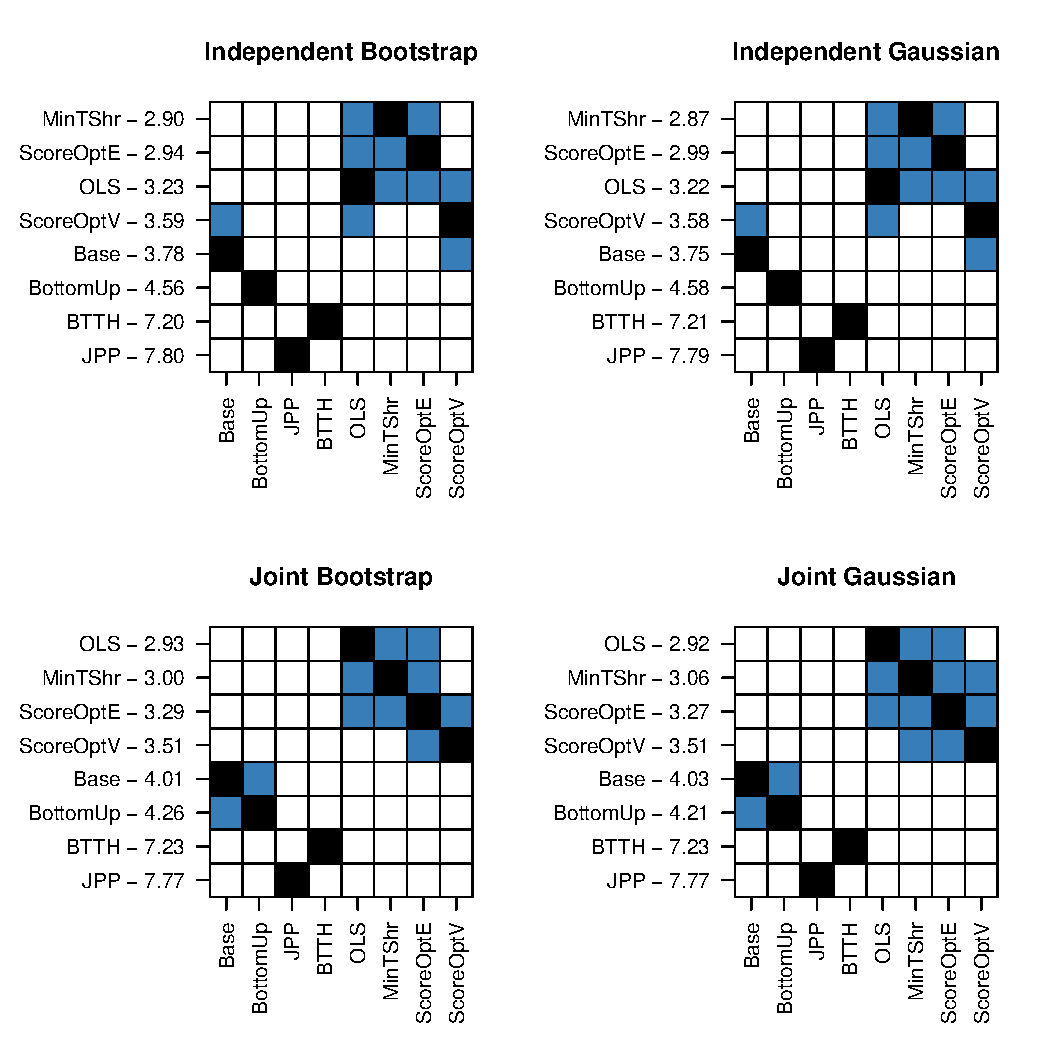
\includegraphics[width=.6\textheight]{Figs/gse.pdf}
	\caption{Nemenyi matrix for Energy Score for Gaussian DGP.}
	\label{fig:gse}
\end{figure}


The right panel of Figure~\ref{fig:meanscore_g} and Figure~\ref{fig:gsv} report the same output but using the variogram score for evaluation. For this specific DGP, base model and score, BTTH significantly outperforms all other methods. However, this result was not observed when using BTTH for any other simulation scenario, including those reported only in the online supplement. Excluding this result, score optimisation with respect to the variogram score is the best performing method with MinTShr and OLS also performing well. Score optimisation, OLS, MinTShr and BTTH all lead to significant improvements relative to base, bottom-up and JPP.

\begin{figure}[!htb]
	\centering
	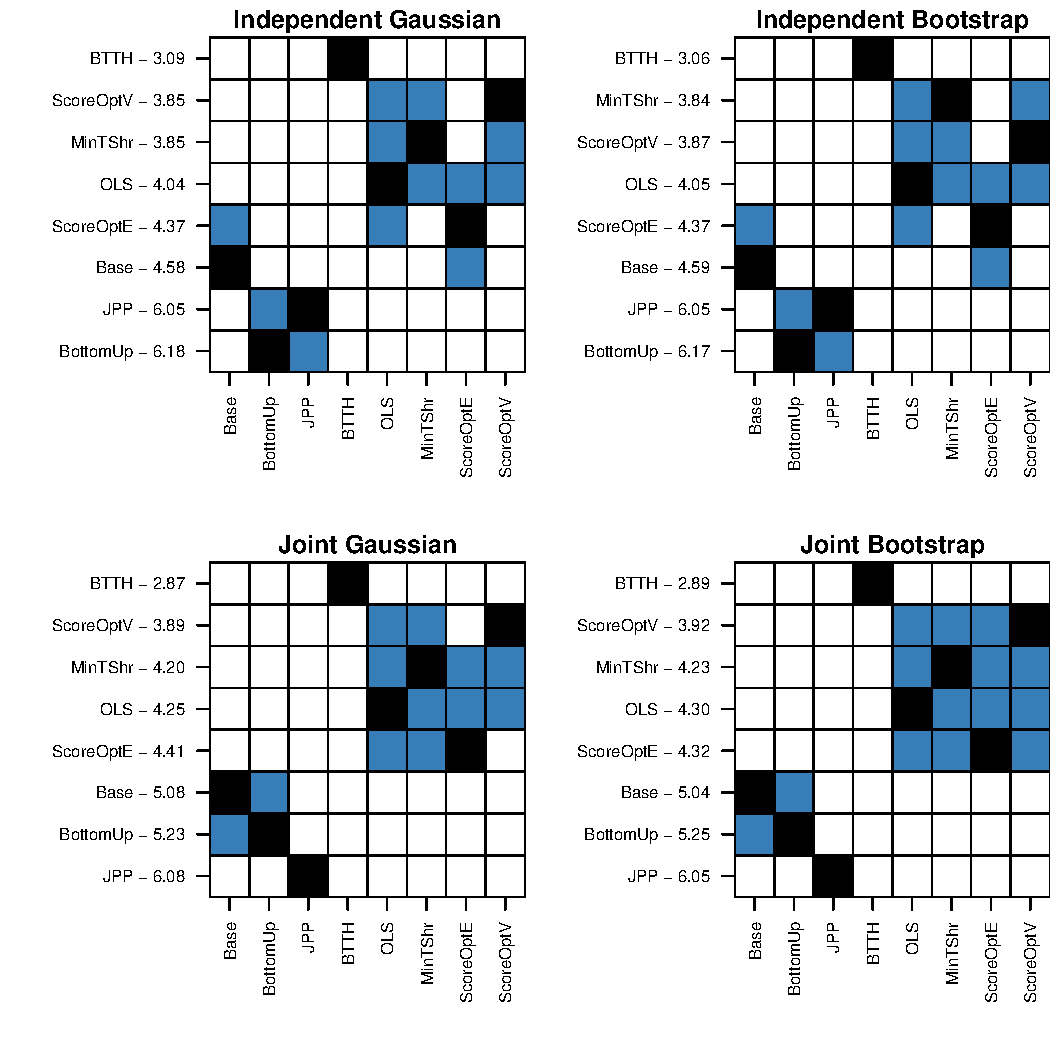
\includegraphics[width=.6\textheight]{Figs/gsv.pdf}
	\caption{Nemenyi matrix for Variogram score for Gaussian DGP.}
	\label{fig:gsv}
\end{figure}

\subsection{Results for non-Gaussian probabilistic forecast} \label{sec:SimSamplingResults}

The left panel of Figure~\ref{fig:meanscore_n} reports the mean energy score for the non-Gaussian DGP\@. Overall, the results are quite similar to the Gaussian DGP\@. The best performing reconciliation method is ScoreOptE when base probabilistic forecasts are independent, and MinTShr when base forecasts are dependent. The Nemenyi matrix is omitted for brevity; please refer to \url{https://git.io/JJwQB} for a full set of results. However, these lead to similar conclusion to Figure~\ref{fig:gse}. The methods ScoreOptE, MinTShr and OLS are statistically indistinguishable from one another but are significantly better than base forecasts and the bottom-up method. The methods BTTH and JPP lead to a statistically significant deterioration in forecast quality relative to base forecasts.

Finally, the right panel of Figure~\ref{fig:meanscore_n} and Figure~\ref{fig:nsv} report results for the non-Gaussian DGP using the variogram score to evaluate forecasts. In this case, score optimisation with respect to the variogram score yields the best performance when base forecasts are dependent, while MinTShr yields the best performance when base forecasts are independent. In contrast to the Gaussian DGP, the JPP method leads to significant improvements over base forecasts, while the BTTH method leads to a significantly worse performance than base forecasts.

\begin{figure}[!htb]
	\centering
	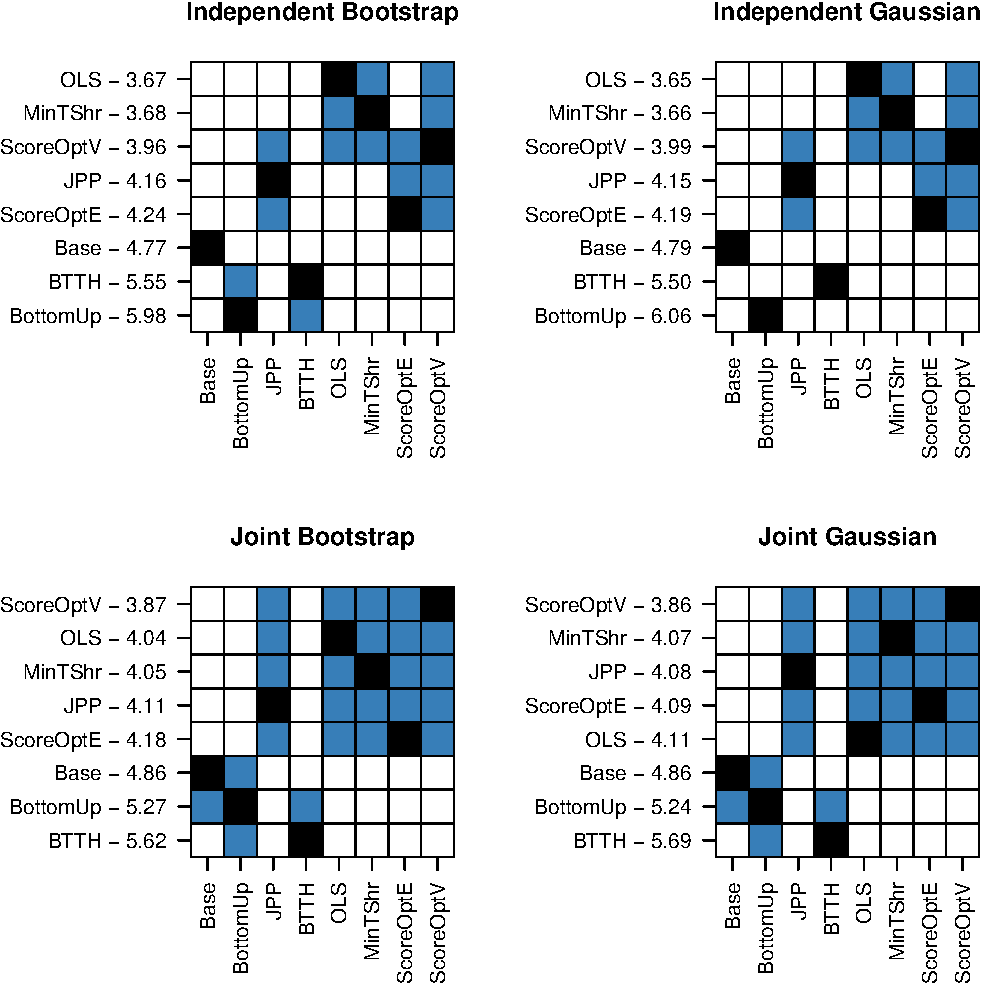
\includegraphics[width=.6\textheight]{Figs/nsv.pdf}
	\caption{Nemenyi matrix for Variogram score with a non-Gaussian DGP.}
	\label{fig:nsv}
\end{figure}

Overall, the main conclusion from the simulation study is that score optimisation leads to significant improvements in forecast performance over base forecasts irrespective of whether the DGP is Gaussian or non-Gaussian and irrespective of whether the energy or variogram score is used for evaluation. For the DGPs considered in the simulation study, MinTShr and to a lesser extent OLS also provided significant improvements over base and bottom-up forecasts. While the existing probabilistic forecast reconciliation methods considered in the literature (BTTH and JPP) performed well in some scenarios (particularly BTTH for the Gaussian DGP evaluated by variogram score), overall results for these methods was mixed and even led to a statistically significant deterioration in forecast quality relative to base forecasts in some settings.

\section{Forecasting Australian Electricity Generation}\label{sec:Application}

\subsection{Data Description}\label{sec:datadesc}

To demonstrate the potential of the proposed methods, we consider an application to forecasting Australian electricity generation from different sources of energy. Daily time series were obtained from \url{opennem.org.au}, a website that compiles publicly available data from the Australian Energy Market Operator (AEMO)\@. Probabilistic day-ahead forecasts are crucial inputs into operational and planning decisions that ensure the efficiency and stability of the power network. This has become a more challenging problem with the growth in intermittent sources of generation such as wind and solar.

The hierarchy comprises three levels of aggregation.
\begin{compactenum}
	\item \textit{Total} generation is the sum of generation from \textit{Renewable} and \textit{non-Renewable} sources.
	\item \textit{Renewable} generation is the sum of \textit{Batteries}, \textit{Hydro (inc. Pumps)}, \textit{Solar}, \textit{Wind} and \textit{Biomass}. \textit{Non-Renewable} is the sum of \textit{Coal}, \textit{Gas} and \textit{Distillate}
	\item \textit{Battery} generation is given by \textit{Battery (Discharging)} minus \textit{Battery (Charging)}, \textit{Hydro (inc. Pumps)} is \textit{Hydro} generation minus \textit{Pumps} (energy used to pump water upstream), while \textit{Solar} generation is the sum of \textit{Solar (Rooftop)} and \textit{Solar (Utility)}. \textit{Coal} generation is the sum of \textit{Black Coal} and \textit{Brown Coal}, while \textit{Gas} is the sum of \textit{Gas (OCGT)}, \textit{Gas (CCGT)}, \textit{Gas (Steam)}, \textit{Gas (Reciprocating)}.
\end{compactenum}
In total, there are $n=23$ series of which $m=15$ are bottom-level series.


\begin{figure}[!b]
	\centering
	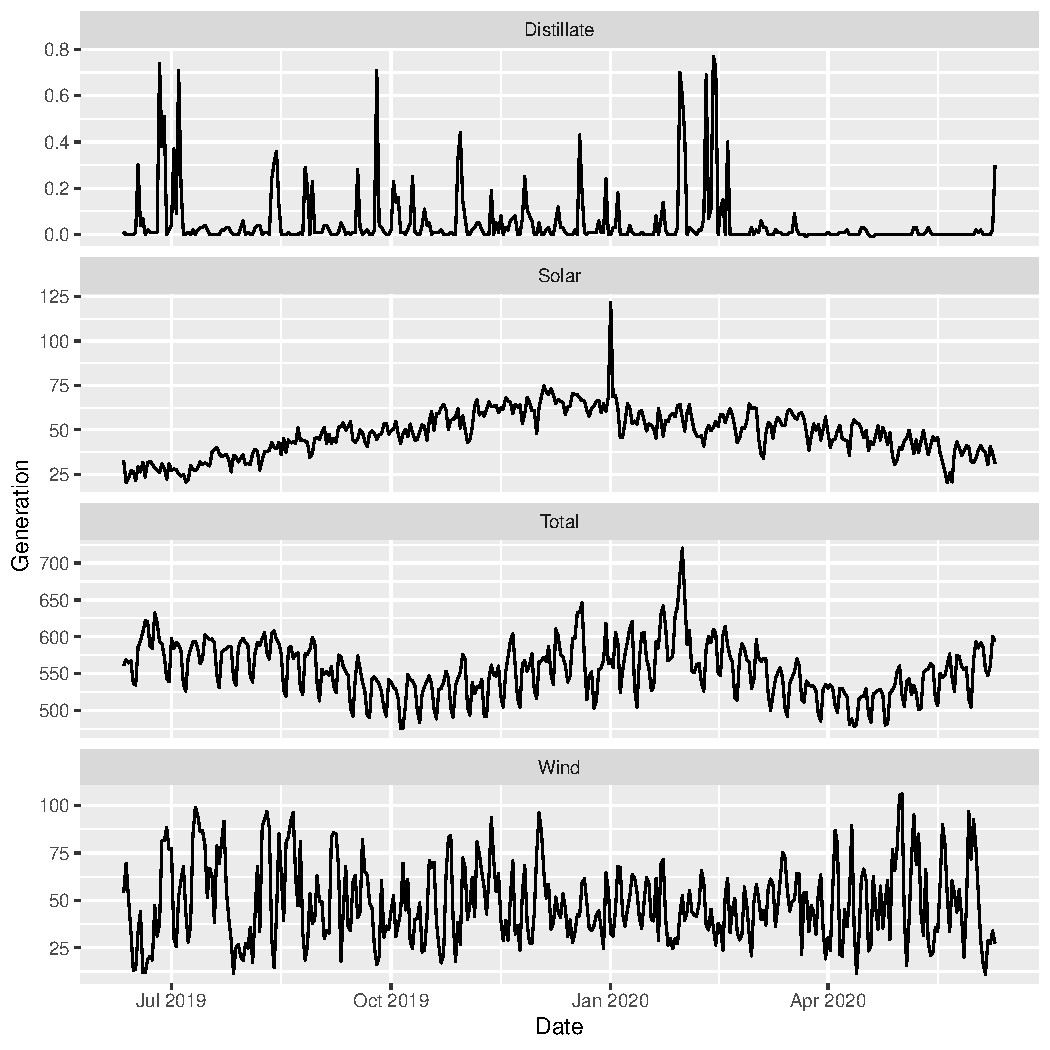
\includegraphics[width=.90\textwidth]{Figs/selected.pdf}
	\caption{Time series plots for selected series from 11 June 2019 to 10 June 2020.}
	\label{fig:selected}
\end{figure}

Figure~\ref{fig:selected} shows time plots for some selected series\footnote{Time plots for the remaining series area available from \url|https://git.io/JJwd0|.}. The series exhibit some interesting and unique features. At the aggregate level, \textit{Total} generation shows strong weekly seasonality, with troughs corresponding to weekends. An annual seasonal pattern is also displayed with peaks occurring during the months of June--August as well as December--February. These periods correspond to the winter and summer months in Australia for which electricity demand peaks for heating and cooling purposes respectively. As expected, generation from \textit{Solar} peaks during the summer months of December--February. There are also some unusually large spikes observed in both the \textit{Total} and \textit{Solar} series during February and January 2020 respectively. \textit{Wind} displays higher volatility (especially outside the summer months), while generation from \textit{Distillate} exhibits aperiodic spikes.

The diversity and prominence of the features in each series and each level of aggregation highlights the importance of modelling and forecasting each series on its own merits and then applying a reconciliation approach.

\subsection{Base Forecasts}\label{sec:applbase}

The forecast evaluation is based on a rolling window. Each training window consists of 140 days (20 weeks) of data. One-step-ahead forecasts were generated leading to 170 daily forecasts for evaluation. Each series was independently modelled using a one-layer feed-forward neural network with up to 28 lags of the target variable as inputs. This was implemented using the \verb|NNETAR| function in the \verb|fable| package. Neural networks are used to highlight the versatility of reconciliation to different forecasting approaches. While including more layers or meteorological variables as predictors will probably lead to improved base forecasts, the primary objective is to assess the effectiveness of different forecast reconciliation methods.

\begin{figure}[!htb]
	\centering
	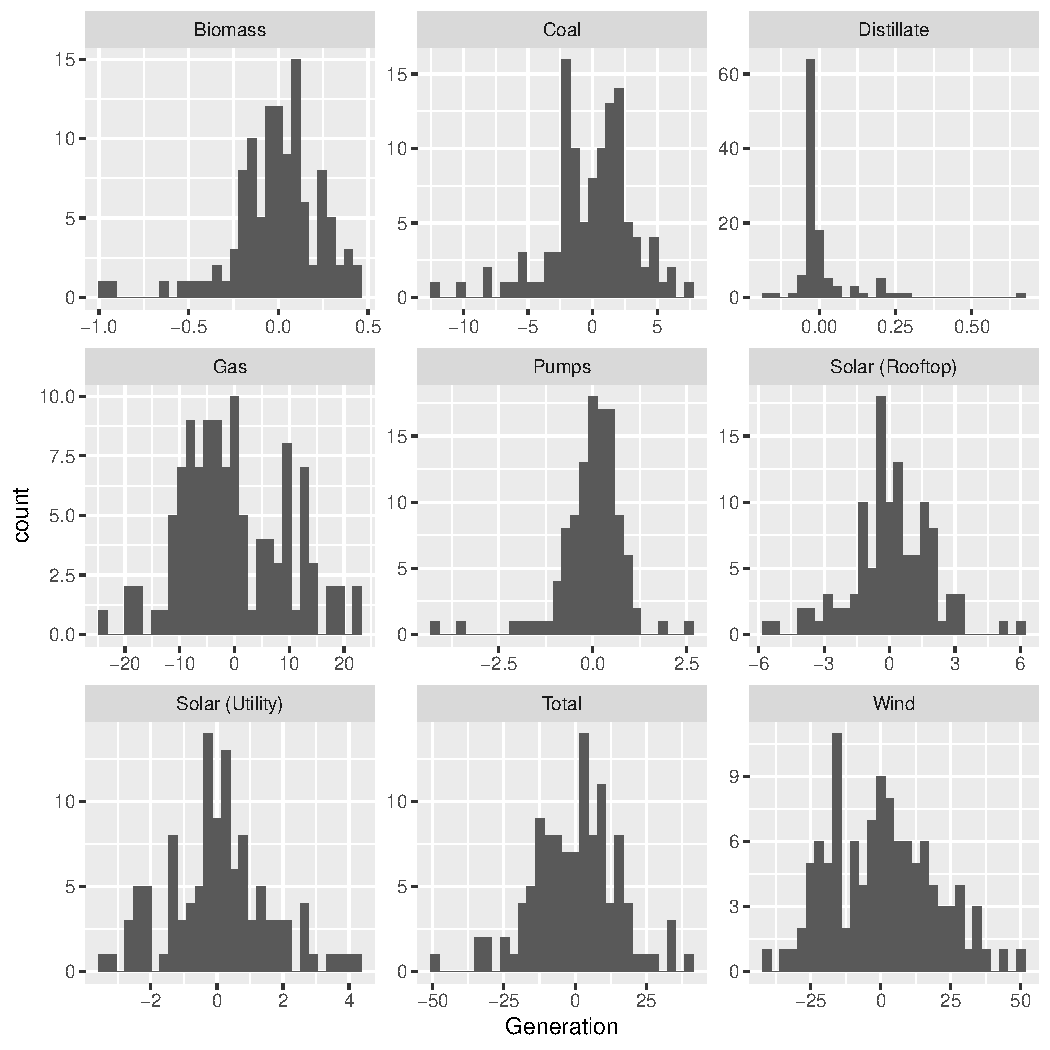
\includegraphics[width=.8\textwidth]{Figs/densities.pdf}
	\caption{Densities of residuals for selected series from a typical training window of 2 October 2019 to 21 January 2020.}
	\label{fig:emp_hist}
\end{figure}

\begin{figure}[!htb]
	\centering
	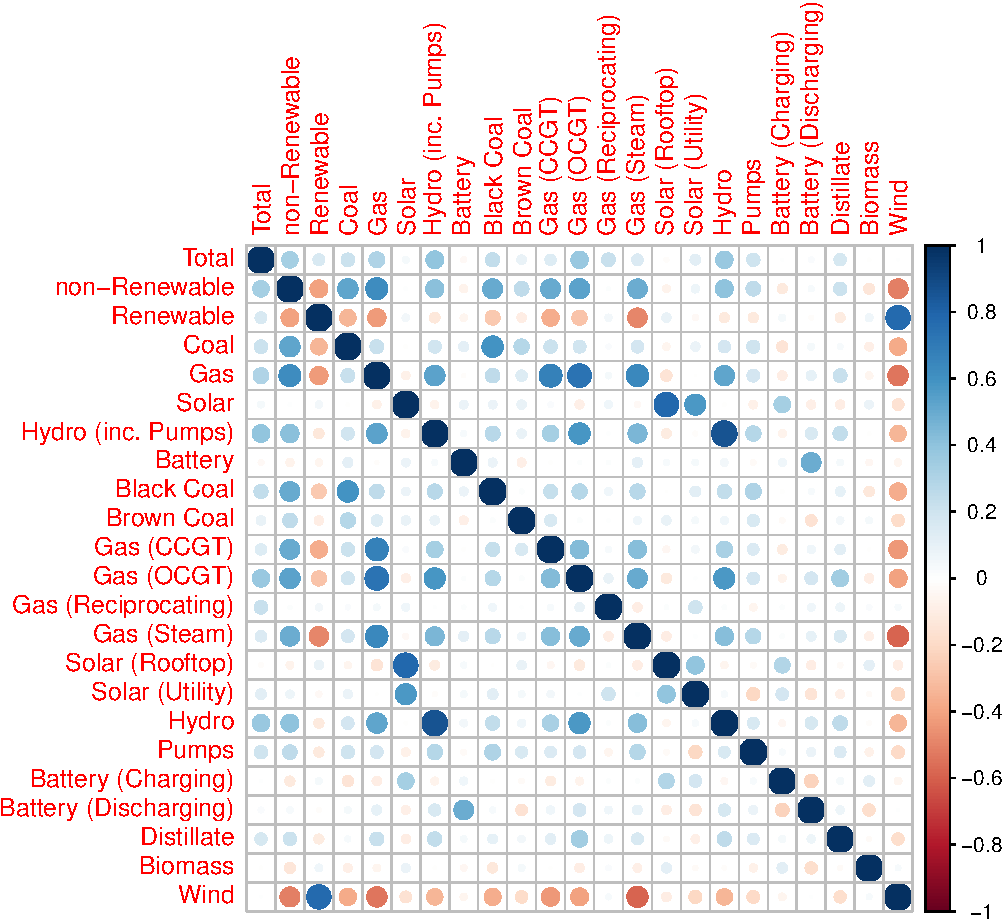
\includegraphics[width=.8\textwidth]{Figs/corr.pdf}
	\caption{Correlation heatmap of residuals from a typical training window of 2 October 2019 to 21 January 2020. Blue circles indicate positive correlation, while red circles indicate negative correlation with larger circles indicating stronger correlations.}
	\label{fig:emp_corr}
\end{figure}

Four situations were considered where base forecasts are assumed to be either Gaussian or bootstrapped from residuals, and either dependent or independent. The histograms in Figure~\ref{fig:emp_hist} demonstrate departures from normality while the correlation heatmap in Figure~\ref{fig:emp_corr} demonstrates departures from independence. Therefore, independent Gaussian probabilistic forecasts are likely to represent a case of severe misspecification.

\subsection{Reconciliation}\label{sec:applreco}

The same methods were used for reconciliation as in the simulation study with score optimisation based on an objective function containing 56 days (8 weeks) of score evaluations. For brevity, only the results for energy score are presented here; please refer to \url{https://git.io/JJwQB} for a full set of results.

\begin{figure}[!htb]
	\centering
	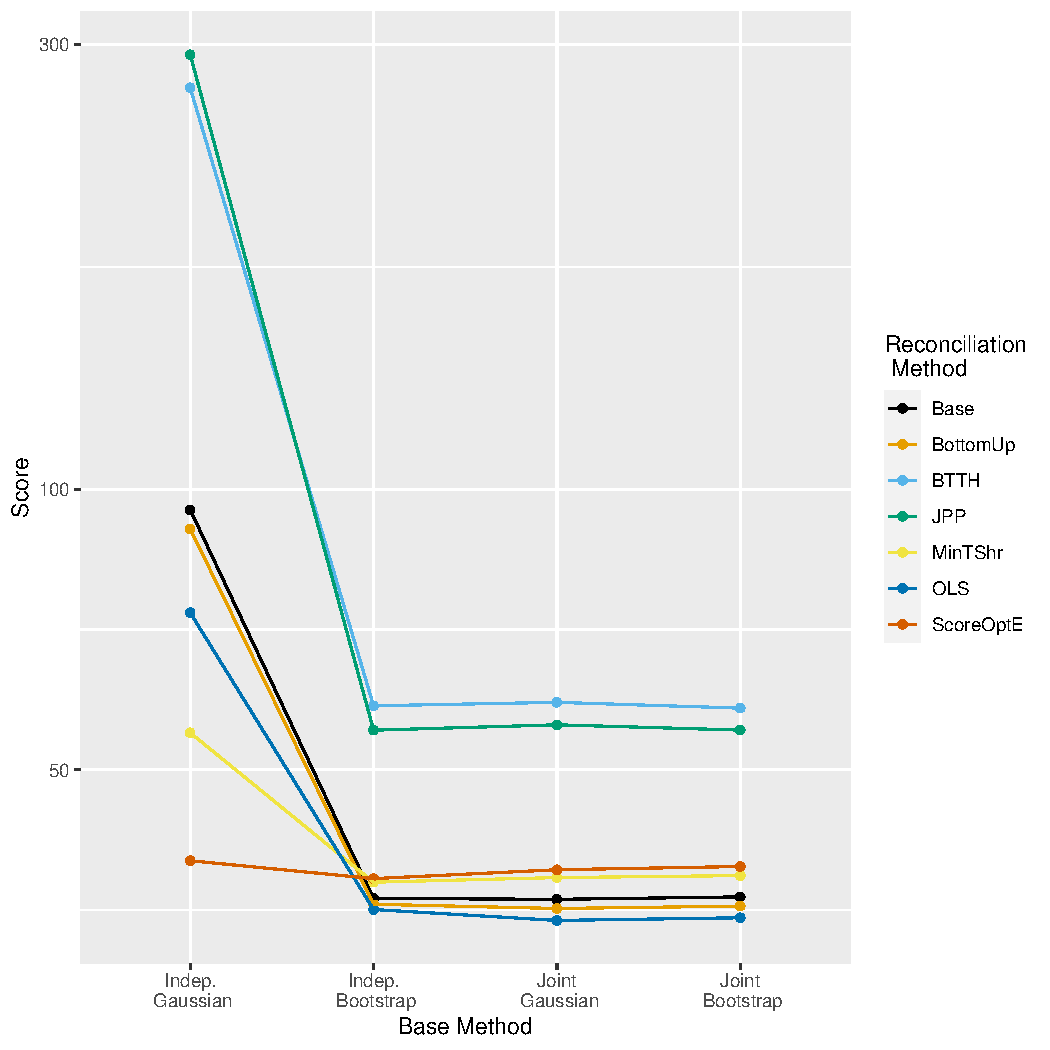
\includegraphics[width=.7\textwidth]{Figs/meanenergyscore}
	\caption{Mean Energy score for the electricity application for different base forecasting methods and different reconciliation methods}\label{fig:meanenergy_app}
\end{figure}

\begin{figure}[!htb]
	\centerline{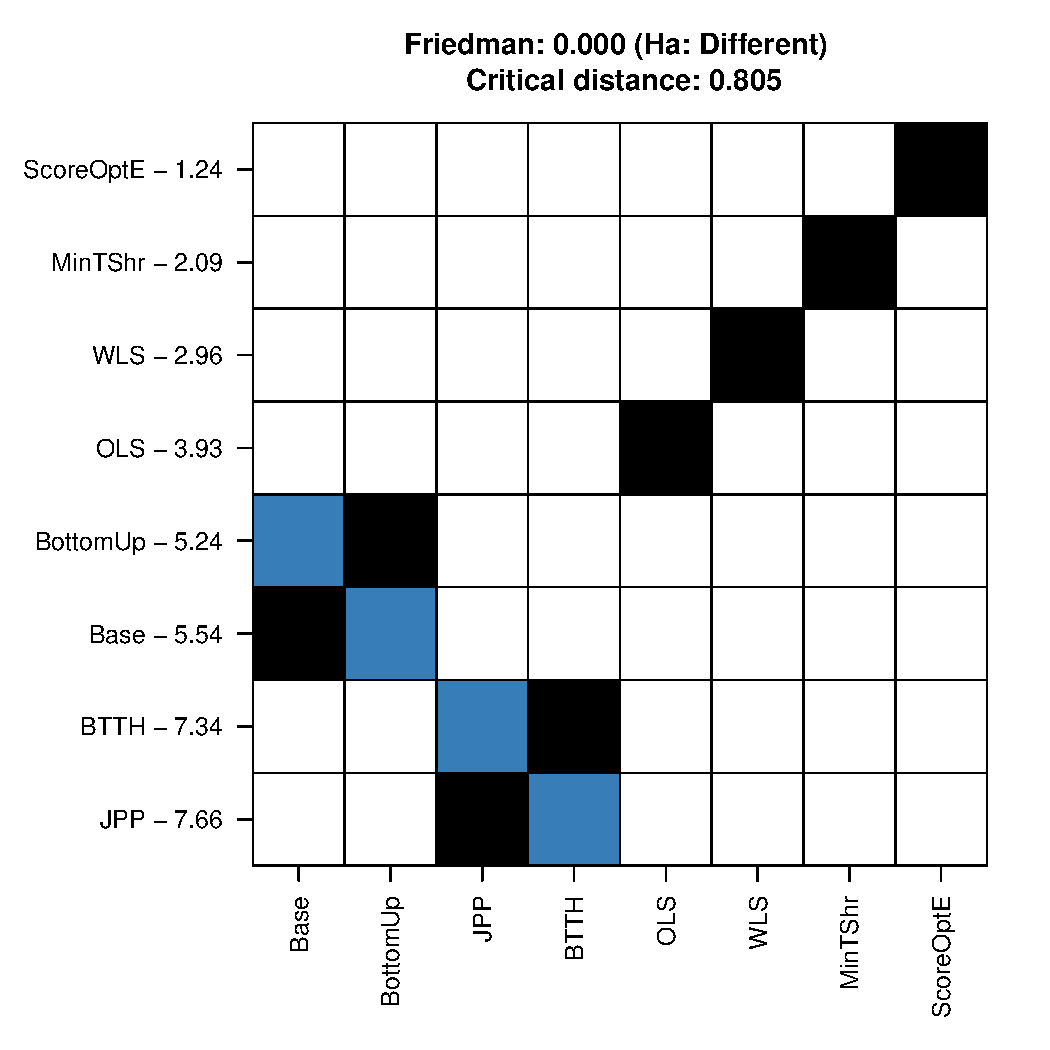
\includegraphics[width=.45\textwidth]{Figs/nemenyi_ig.pdf}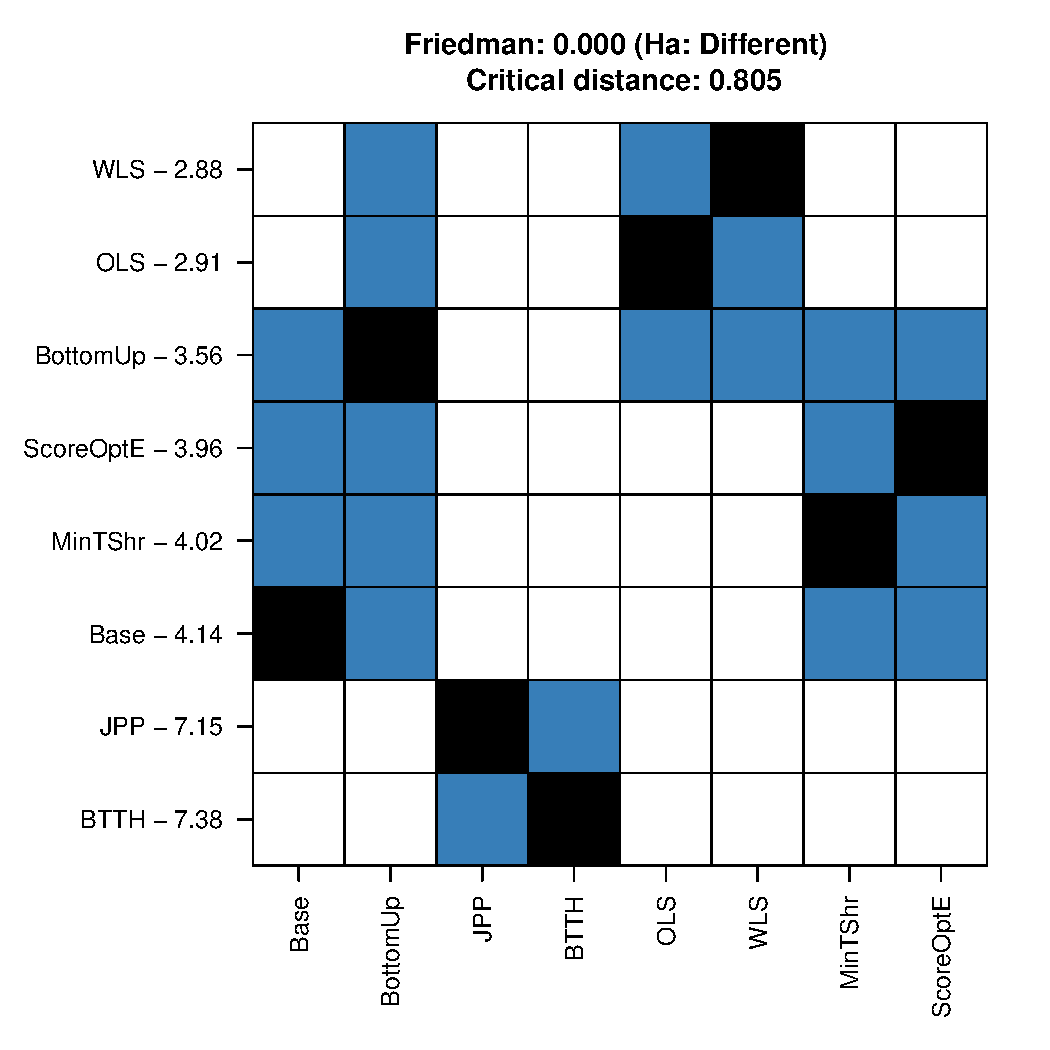
\includegraphics[width=.45\textwidth]{Figs/nemenyi_jb.pdf}}
	\caption{Nemenyi matrices for Energy score for the electricity application. Left: base forecasts are independent and Gaussian. Right: base forecasts are obtained by jointly bootstrapping residuals.}\label{fig:nem_app}
\end{figure}

The mean energy score for all four base forecasting methods is summarised in Figure~\ref{fig:meanenergy_app}. When base forecasts are generated assuming both independence and a Gaussian distribution, score optimisation achieves a mean energy score that is considerably smaller than all other competing methods, with MinT providing the second smallest value. Figure~\ref{fig:nem_app} (left) provides the Nemenyi matrix for this set of base forecasts, and shows that the superior forecasting performance of score optimisation is statistically significant. This suggests that score optimisation is best for guarding against severe model misspecification.

For all other methods the best performing method is OLS. This difference is statistically significant as seen in Figure~\ref{fig:nem_app} (right), which shows the Nemenyi matrix for jointly bootstrapped base forecasts. The corresponding figures for joint Gaussian and independent bootstrap look mostly similar to the right panel of Figure~\ref{fig:nem_app}; please refer to \url{https://git.io/JJwQB} for a full set of results. Although score optimisation does not improve upon base, the differences are not significant. For all base forecasts, both JPP and BTTH are significantly worse than base forecasts.


\section{Conclusions}\label{sec:conclusion}

This paper introduces a rigorous formulation of forecast reconciliation in the probabilistic setting. It can be applied when the probabilistic forecast is either available as a density or when a sample has been drawn from the probabilistic forecast. In the elliptical case, we prove that reconciliation can recover the correct probability distribution as long as the base forecast is of the correct form, irrespective of the scale and location of the base forecast. Probably due to this reason, score optimisation works well in applications even when the base forecasts are assumed to be independent.

We also prove that the log score is not proper when comparing incoherent and coherent forecasts. Consequently, we introduce a new algorithm that trains reconciliation weights by minimising the energy score or variogram score. Since the scores are approximated by Monte Carlo simulation, stochastic gradient descent is used for optimisation. This method is shown to lead to significant improvements over base forecasts, bottom-up methods and existing probabilistic reconciliation approaches across a wide variety of simulated and empirical examples.

An interesting result is that projection methods with certain optimality properties in the point forecasting setting, also work well when extended to the probabilistic case. In particular, a simple least squares projection is the best performing method in the high-dimensional empirical example, provided the base forecasts are not too badly misspecified. This may arise since projections implicitly provide constrained versions of the reconciliation weights. A promising future research avenue may involve regularised versions of score optimisation that add an $L_1$ or $L_2$ penalty to the objective function. Alternatively, early stopping \citep{BuhYu2003,YaoEtAl2007} of the gradient descent may lead to a better bias-variance tradeoff in learning reconciliation weights.

A final important avenue of future research is the development of probabilistic forecast reconciliation for domains other than the real line. These may include domains constrained above zero, discrete domains, or domains that are a mixture of continuous distributions and discrete point masses. While such problems are challenging, the geometric interpretation of probabilistic forecast introduced in this paper, lays the foundation for this research agenda.

\clearpage

\appendix

\section{Proof of Theorem~\ref{theo:bottomdens} and Theorem~\ref{theo:fulldens}} \label{app:Bottom&FullDens}

Consider the region $\mathcal{I}$ given by the Cartesian product of intervals $(l_1,u_1),(l_2,u_2),\ldots(l_m,u_m)$. We derive the probability, under the reconciled measure, that the bottom-level series lie in $\mathcal{I}$, i.e. $\mbox{Pr}(\bm{\ell}\succ\bm{b}\succ\bm{u})$, where $\bm{\ell}=(\ell_1,\ell_2,\ldots,\ell_m)$, $\bm{u}=(u_1,u_2,\ldots,u_m)$ and $\succ$ denotes element-wise inequality between vectors. The pre-image of $\mathcal{I}$ under $g$ can similarly be denoted as all points $\bm{y}$ satisfying $\bm{\ell}\succ\bm{G}\bm{y}\succ\bm{u}$. Using Definition~\ref{def:reconprob},
\[
\mbox{Pr}(\bm{\ell}\succ\bm{b}\succ\bm{u})=\int\limits_{\bm{\ell}\succ\bm{G}\bm{y}\succ\bm{u}}\hat{f}(\bm{y})d\bm{y}\,,
\]
where $\hat{f}$ is the density of the base probabilistic forecast. Now consider a change of variables to an $n$-dimensional vector $\bm{z}$ where $\bm{y}=\bm{G}^*\bm{z}$. Recall, $\bm{G}^*=\big(\bm{G}^{-}\,\vdots\,\bm{G}_\perp\big)$, $\bm{G}^{-}$ is a generalised inverse of $\bm{G}$, and $\bm{G}_\perp$ is an orthogonal complement of $\bm{G}$. By the change of variables

\begin{align}
	\mbox{Pr}(\bm{\ell}\succ\bm{b}\succ\bm{u})&=\int\limits_{\bm{\ell}\succ\bm{G}\bm{y}\succ\bm{u}}\hat{f}(\bm{y})d\bm{y}\nonumber\\
	&=\int\limits_{\bm{\ell}\succ\bm{G}\bm{G}^*\bm{z}\succ\bm{u}}\hat{f}(\bm{G}^*\bm{z})|\bm{G}^*|d\bm{z}\nonumber\\
	&=\int\limits_{\bm{\ell}\succ\bm{z}_1\succ\bm{u}}\hat{f}(\bm{G}^*\bm{z})|\bm{G}^*|d\bm{z}\nonumber\,,
\end{align}
where $\bm{z}_1$ denotes the first $m$ elements of $\bm{z}$. Letting $\bm{a}$ denote the last $n-m$ elements of $\bm{z}$ the integral above can be written as
\[
\mbox{Pr}(\bm{b}\in \mathcal{I})=\int\limits_{\bm{\ell}\succ\bm{z}_1\succ\bm{u}}\!\!\!\!\!\int\hat{f}(\bm{G}^{-}\bm{z}_1+\bm{G}_{\perp}\bm{a})|\bm{G}^*|d\bm{a}d\bm{z}_1\nonumber\\
\]
Replacing $\bm{z}_1$ with $\bm{b}$, it can be seen that the term inside the outer integral is a density for the bottom-level series. Therefore

\begin{equation}
\tilde{f}_{\bm{b}}(\bm{b})=\int\hat{f}(\bm{G}^{-}\bm{b}+\bm{G}_{\perp}\bm{a})|\bm{G}^*|d\bm{a}\,,
\label{eq:densb}
\end{equation}
is the density of $\bm{b}$. To obtain the density of the full hierarchy we first augment the density in Equation \eqref{eq:densb} by $n-m$ variables denoted $\bm{u}$

\begin{equation}
f(\bm{b},\bm{u})=\tilde{f}_b(\bm{b})\mathbb{1}\{\bm{u}=0\}\,,
\end{equation}
such that the density $f(\bm{b},\bm{u})$ is a density for $n$-dimensional vector that is degenerate across the dimensions corresponding to $\bm{u}$. Using the change of variables,
\[
\bm{y}=\big(\bm{S}\,\vdots\,\bm{S}^-_{\perp}\big)\bigg(\begin{matrix}\bm{b}\\[-0.3cm]
\bm{u}
\end{matrix}\bigg)\,,
\]
where $\bm{S}^-_{\perp}$ is a generalised inverse such that $\bm{S}'_{\perp}\bm{S}^-_{\perp}=\bm{I}$ and noting the inverse of $\big(\bm{S}\,\vdots\,\bm{S}_{\perp}\big)$ is given by
\[
\bm{S}^*:=\bigg(\begin{matrix}\bm{S}^{-}\\[-0.2cm]\bm{S}'_{\perp}\end{matrix}\bigg)\,,
\]
it can be seen that $\bm{b}=\bm{S}^-\bm{y}$ and $\bm{u}=\bm{S}'_\perp\bm{y}$. Applying this change of variables yields the density
\[
\tilde{f}_{\bm{y}}(\bm{y})=|\bm{S}^*|\tilde{f}_{\bm{b}}(\bm{S}^-\bm{y})\mathbb{1}\{\bm{S}'_\perp\bm{y}=\bm{0}\}\,.
\]
Since $\bm{S}'_\perp$ is the orthogonal complement of $\bm{S}$ and since the columns of $\bm{S}$ span the coherent subspace, the statement $\bm{S}'_\perp\bm{y}=0$ is equivalent to the statement $\bm{y}\in\mathfrak{s}$. As such, the reconciled density is given by
\[
\tilde{f}_{\bm{y}}(\bm{y})=|\bm{S}^*|\tilde{f}_b(\bm{S}^-\bm{y})\mathbb{1}\{\bm{y}\in\mathfrak{s}\}.
\]

\clearpage

\section{Proof of Theorem~\ref{theo:OptRecProj}}
\label{app:OptRecProj}

Let
\[
\hat{\bm{\Sigma}}=\bm{\Sigma}+\bm{D}=\bm{S}\bm{\Omega}{\bm{S}}'+\bm{D}\,.
\]
If reconciliation is carried out via a projection onto $\mathfrak{s}$, then $\bm{S}\bm{G}\bm{S}=\bm{S}$ and
\begin{align}
	\tilde{\bm{\Sigma}}&=\bm{S}\bm{G}\hat{\bm{\Sigma}}\bm{G}'\bm{S}'\nonumber\\
	&\bm{S}\bm{G}\bm{S}\bm{\Omega}\bm{S}'\bm{G}'{\bm{S}}'+\bm{S}\bm{G}\bm{D}\bm{G}'\bm{S}'\nonumber\\
	&\bm{S}\bm{\Omega}{\bm{S}}'+\bm{S}\bm{G}\bm{D}\bm{G}'\bm{S}'\nonumber\\
	&\bm{\Sigma}+\bm{S}\bm{G}\bm{D}\bm{G}'\bm{S}'\nonumber\,.
\end{align}
Therefore to recover the true predictive using a projection, some $\bm{G}_{\text{opt}}$ must be found such that $\bm{G}_{\text{opt}}\bm{D}=\bm{0}$. Let the eigenvalue decomposition of $\bm{D}$ be given by $\bm{R}\bm{\Lambda}\bm{R}'$ , where $\bm{R}$ is an $n\times q$ matrix with $q=\textrm{rank}({\bm{D}})$ and ${\bm\Lambda}$ is an $q\times q$ diagonal matrix containing non-zero eigenvalues of $\bm{D}$. By the rank nullity theorem, $\bm{R}$ will have an orthogonal complement $\bm{R}_{\perp}$ of dimension $n\times (n-q)$. If $q=n-m$ then the number of columns of $\bm{R}_{\perp}$ is $m$ and $\bm{G}_{\text{opt}}$ can be formed as the $m\times n$ matrix $(\bm{R}_{\perp}'\bm{S})^{-1}\bm{R}_{\perp}'$. If $q<n-m$ the number of columns of $\bm{R}_{\perp}$ is greater than $m$, and any $m$ columns of $\bm{R}_{\perp}$ can be used to form $\bm{G}_{\text{opt}}$ in a similar fashion. However when $q>n-m$, the number of columns of $\bm{R}_{\perp}$ is less than $m$ and no such $m\times n$ matrix $\bm{G}_{\text{opt}}$ can be formed. Therefore the true predictive can only be recovered via a projection when $\textrm{rank}(\bm{D})\leq n-m$.

With respect to the location, if $\bm{S}\bm{G}$ is a projection then reconciled forecasts will be unbiased as long as the base forecasts are also unbiased. When base forecasts are biased they can be bias corrected before reconciliation as described by \cite{PanEtAl2020_Geometry} in the point forecasting setting.

\clearpage

\section{Proof of Theorem~\ref{theo:logS_improp}}\label{app:logS_improp}

The proof relies on the following change of variables,
\[
\bm{y}=\big(\bm{S}\,\vdots\,\bm{S}_\perp\big)\bigg(\begin{matrix}\bm{b}\\\bm{u}\end{matrix}\bigg).
\]
Also recall from the proof of Theorem~\ref{theo:fulldens} that $\bm{S}^*=\big(\bm{S}\,\vdots\,\bm{S}_\perp\big)^{-1}$

Let the density of the true predictive $f(\bm{y})$ after a change of variables, be given by $|\bm{S}^*|^{-1}f_{\bm{b}}(\bm{b})\mathbb{1}\{\bm{u}=\bm{0}\}$. To prove that the log score is improper we construct an incoherent base density $\hat{f}$ such that $E_f\big[LS(\hat{f},\bm{y})\big]<E_f\left[LS\left(f,\bm{y}\right)\right]$. This incoherent density is constructed, so that after the same change of variables it can be written as $|\bm{S}^*|^{-1}\hat{f}_{\bm{b}}(\bm{b})\hat{f}_{\bm{u}}(\bm{u})$. We require $\hat{f}_{\bm{u}}(\bm{0})>1$, i.e., $\bm{u}$ is highly concentrated around $\bm{0}$ but still non-degenerate. An example is an independent normal with mean 0 and variance less than $(2\pi)^{-1}$. Now, let $\bm{y}^*$ be a realisation from $f$. Let the first $m$ elements of $\bm{S}^*\bm{y}^*$ be $\bm{b}^*$, and the remaining elements be $\bm{u}^*$. The log score for $f$ is thus,
\begin{align}
	LS\left(f,\bm{y}^*\right) &= -\log f(\bm{y}^*) \nonumber\\
	&=-\log|\bm{S}^*|-\log f_{\bm{b}}\left(\bm{b}^*\right)-\log\left(\mathbb{1}\{\bm{u}^*=\bm{0}\}\right)\label{eq:diraccancel}\\
	&=-\log|\bm{S}^*|-\log f_{\bm{b}}\left(\bm{b}^*\right),\nonumber
\end{align}
where the third term in Equation~\eqref{eq:diraccancel} is equal to zero since the fact that $\bm{y}^*\in\mathfrak{s}$ implies that $\bm{u}^*=\bm{0}$. The log score for $\hat{f}$ is
\[
LS(\hat{f},\bm{y}^*) = -\log|\bm{S}^*|-\log f_{\bm{b}}(\bm{b}^*)- \log f_{\bm{u}}(\bm{0})\,.
\]
Since $f_{\bm{u}}(\bm{0})>1$ by construction, $-\log f_{\bm{u}}(\bm{0})<0$, therefore
\[
LS(\hat{f},\bm{y}^*) <-\log|\bm{S}^*|-\log f_{\bm{b}}(\bm{b}^*)=LS\left(f,\bm{y}^*\right)
\]
Since this holds for any possible realisation, it will also hold after taking expectations (by the monotonicity of expectations). Thus $\hat{f}$ violates the condition for a proper scoring rule.

\clearpage

\section{Data generating process} \label{app:DGP}

To ensure that bottom-level series are noisier than top level series (a feature often observed empirically), noise is added to the bottom-level series in the following manner
\begin{align*}
	y_{AA,t} &= w_{AA,t} + u_t - 0.5v_t,\\
	y_{AB,t} &= w_{AB,t} - u_t - 0.5v_t,\\
	y_{BA,t} &= w_{BA,t} + u_t + 0.5v_t,\\
	y_{BB,t} &= w_{BB,t} - u_t + 0.5v_t,
\end{align*}
where $w_{AA,t},w_{AB,t},w_{BA,t},w_{BB,t}$ are generated from ARIMA processes as described in Section~\ref{sec:dgp} with innovations $\varepsilon_{AA,t},\varepsilon_{AB,t},\varepsilon_{BA,t},\varepsilon_{BB,t}$. 

For the Gaussian DGP, $u_t \sim \mathcal{N}(0,\sigma^2_u)$ and $v_t \sim \mathcal{N}(0,\sigma^2_v)$ and $\{\varepsilon_{AA,t},\varepsilon_{AB,t},\varepsilon_{BA,t},\varepsilon_{BB,t}\} \overset{iid}{\sim} \mathcal{N}(\bm{0}, \bm{\Sigma})~\forall t$. We follow \cite{WicEtAl2019} and set
\begin{equation*}\label{eq:SigmaGaussian}
	\bm{\Sigma} =
	\begin{pmatrix}
		5.0 & 3.1 & 0.6 & 0.4 \\
		3.1 & 4.0 & 0.9 & 1.4 \\
		0.6 & 0.9 & 2.0 & 1.8 \\
		0.4 & 1.4 & 1.8 & 3.0 \\
	\end{pmatrix}
\end{equation*} and $\sigma^2_u=28$ and $\sigma^2_v=22$. This ensures that the following inequalities are satisfied,
\begin{align*}
	\var(\varepsilon_{AA,t} + \varepsilon_{AB,t} + \varepsilon_{BA,t} + \varepsilon_{BB,t})
	\le \var(\varepsilon_{AA,t}+\varepsilon_{AB,t}-v_t)
	\le \var(\varepsilon_{AA,t}+u_t-0.5v_t),\\
	\var(\varepsilon_{AA,t} + \varepsilon_{AB,t} + \varepsilon_{BA,t} + \varepsilon_{BB,t})
	\le \var(\varepsilon_{AA,t}+\varepsilon_{AB,t}-v_t)
	\le \var(\varepsilon_{AB,t}-u_t-0.5v_t),\\
	\var(\varepsilon_{AA,t} + \varepsilon_{AB,t} + \varepsilon_{BA,t} + \varepsilon_{BB,t})
	\le \var(\varepsilon_{BA,t}+\varepsilon_{BB,t}+v_t)
	\le \var(\varepsilon_{BA,t}+u_t+0.5v_t),\\
	\var(\varepsilon_{AA,t} + \varepsilon_{AB,t} + \varepsilon_{BA,t} + \varepsilon_{BB,t})
	\le \var(\varepsilon_{BA,t}+\varepsilon_{BB,t}+v_t)
	\le \var(\varepsilon_{BB,t}-u_t+0.5v_t).\\
\end{align*}

For the non-Gaussian case, errors are generated from a Gumbel copula with Beta margins as described in Section~\ref{sec:dgp}. Rather than add Gaussian noise, we simulate $u_t$ and $v_t$ from skew t distributions using the \texttt{sn} package \citep{snpackage}. The scale, skew and degrees of freedom parameters are chosen as 0.5,1.5 and 4 and 0.9,2 and 8 for $u_t$ and $v_t$ respectively. Monte Carlo simulations show that these values satisfy the inequalities described above.


\clearpage

\bibliographystyle{agsm}

\bibliography{References_paper2}

\end{document}